%% IEEE VIS 2027 / VAST Track — VGTC Conference Paper (double-blind review submission)
\documentclass[journal,review]{vgtc}

\usepackage{cite}
\usepackage{graphicx}
\usepackage{amsmath}
\usepackage{amssymb}
\usepackage{amsthm}
\usepackage{booktabs}
\usepackage{array}
\usepackage{multirow}
\usepackage{xcolor}
\usepackage{listings}
\usepackage{microtype}
\graphicspath{{figures/}{docs/figures/}}
\raggedbottom

%% VGTC paper metadata
\onlineid{0}

\vgtccategory{Research}

\title{ConceptGrade: A Visual Analytics System for Human-AI Co-Auditing of Knowledge Graph-Grounded Grading}

\author{Anonymous Submission}
\authorfooter{Anonymous submission for double-blind review.}

\shortauthortitle{ConceptGrade: VA for Grading Co-Auditing}

\abstract{%
\textbf{Correction notice (2026-07-28): the Mohler-specific ML-accuracy numbers throughout this paper --- the $1{,}134$/$177$-question pool, $32.4\%$/$34.0\%$ MAE reductions, $n=90$/$n=120$ splits, the component-ablation table, and the TRM grounding-density analysis --- were computed against a fabricated 120-sample fixture, not the real Mohler et al.\ (2011) benchmark; see the companion paper's REPRODUCIBILITY.md for the full incident record. This Abstract and the ML-accuracy section (\S\ref{sec:evaluation_accuracy}) now report the corrected, real-data result ($n=1{,}262$, 46 questions, $8.2\%$ MAE reduction, response-level significant but only question-level-marginal). The component ablation and TRM grounding-density tables require new pipeline runs on real data and are reported as open future work rather than carried forward.}
Knowledge-graph-grounded automated short-answer grading systems are a maturing class of architectures, but their effectiveness depends sharply on how well the KG covers the domain vocabulary of the answers being graded. The same KG-grounded scoring pipeline can be near-instructor-grade on in-domain answers and silently miscalibrated on adjacent-domain or out-of-domain answers --- and the educator using it currently has no actionable interface for distinguishing the two regimes per-answer. This paper contributes a visual analytics design for that specific operational problem: \emph{structural-confidence triage} in cross-domain KG-grounded ASAG. We present ConceptGrade Dashboard, a system that surfaces three architectural reliability signals --- the topological-continuity of the LLM's reasoning over the KG, the agreement between the KG-coverage signal and the LLM's confidence, and the upstream concept-extraction grounding density --- as interactive visual affordances. We instantiate and evaluate the dashboard on top of an existing KG-grounded pipeline (ConceptGrade) whose ML accuracy we have separately characterised on three datasets totalling $2{,}276$ unique paired student-answer predictions across $213$ questions (Mohler is the real, corrected data as of 2026-07-28; the Kaggle ASAG source distribution's $473$ records contain $105$ byte-identical duplicates, deduplicated for this figure), finding a small, statistically fragile in-domain effect ($8.2\%$ MAE reduction on the real Mohler 2011 sample, $n=1{,}262$, response-level Wilcoxon two-tailed $p<0.0001$ but question-clustered $p=0.111$, paired $d_z=-0.154$) and explicit cross-domain heterogeneity ($I^2 = 73.2\%$). We report this candidly rather than as a stronger claim: even in its most favourable domain, the underlying ML pipeline's advantage over an identical-model zero-shot LLM baseline is modest and fragile, which if anything strengthens the case for this paper's actual contribution --- a triage interface that helps an educator tell reliable answers from unreliable ones, rather than trusting a single aggregate accuracy number. The dashboard's design treats the heterogeneity (both across datasets and across the reliability of any single grade) as the per-answer triage problem it actually is, not as a system-level limitation: each visual encoding maps to a specific architectural condition under which a structural ASAG pipeline can be reliable, marginal, or fail. A pre-registered controlled study with $N=64$ domain-expert educators is designed to evaluate whether the dashboard's structural-confidence indicators yield higher \emph{silent-failure detection accuracy} --- the regime where numeric summaries provably cannot disambiguate --- than a text-summary baseline. The core technical contribution is the visual encoding of \emph{Topological Reasoning Mapping} projected onto the domain KG, together with the failure-detection user-study design. We argue that the load-bearing gap in deployed KG-grounded ASAG is not a more capable model or a richer feature set, but an interface that lets the educator see, per answer, whether the structural assumptions on which the score depends actually hold.%
}

\keywords{visual analytics, automated grading, knowledge graphs, human-AI collaboration, educator trust, educational data mining}

\newtheorem{definition}{Definition}

\begin{document}

\firstsection{Introduction}
\maketitle

%% NOTE: \firstsection{Introduction} above causes vgtc to auto-generate the
%% first \section heading inside \maketitle. The explicit \section{Introduction}
%% below is intentionally omitted — vgtc handles it via \firstsectiontxt.

%% Body of Introduction:

\noindent\textbf{Submission status: design-and-protocol document,
pre-data-collection.} This paper describes (i)~the ConceptGrade
dashboard's design rationale, (ii)~the pre-registered protocol for a
controlled user study with $N=64$ domain-expert educators, and
(iii)~projected effect sizes from mock data so readers can audit the
analysis plan. \textbf{User-study results are \emph{not} reported in
this paper; this is a design-and-protocol paper, not a completed
empirical evaluation.} All figures in the Results section
(§\ref{sec:evaluation_user_study}) are explicitly labelled
\textsc{Pre-Submission Placeholder} and will be replaced by real data
in a post-collection revision. Empirical claims about ML
grading accuracy on the three datasets (Mohler, DigiKlausur,
Kaggle ASAG) use real cached results computed in the companion paper.
Following five rounds of external expert consultation (recorded as
Gemini-2.5-flash advisory rounds 1--5 in supplementary materials
\texttt{data/gemini\_*\_review.json}), and per the explicit Round-5
terminal verdict that ``peer-reviewed HCI and VIS venues including
workshops and CHI LBR do not accept design papers that feature
explicit placeholders for their primary user studies,'' \textbf{this
manuscript will not be submitted to any peer-reviewed venue in its
present form}. The present version is being released as an
\emph{OSF preprint only} for transparent open-science registration of
the dashboard design and the user-study protocol, anchoring the
pre-registered hypotheses publicly before $N=64$ data collection
begins. A submission-ready manuscript with collected behavioural data
is targeted for IEEE VIS 2028 (or an equivalent peer-reviewed venue)
after the summer 2026 study has been executed and the placeholder
figures are replaced.

Large language models have achieved impressive aggregate accuracy on
short-answer grading tasks~\cite{Liu2024,Wei2023_GEVAL}, and a growing
family of \emph{structural} or \emph{KG-grounded} systems augments
those models with explicit domain-knowledge anchoring to improve
in-domain reliability. But in high-stakes educational contexts a
quieter empirical regularity is the harder problem: \emph{the same
structural ASAG pipeline can be near-instructor-grade on one
answer and silently miscalibrated on the next, even within a single
classroom dataset, and the educator using it has no actionable
per-answer indication of which regime they are in.} The aggregate
accuracy number on the venue benchmark is not the operational
quantity the educator needs.

This paper addresses that gap as a visual analytics design problem.
Concretely, we contribute ConceptGrade Dashboard, a coordinated
multi-view system that surfaces three architectural reliability signals
for each graded answer: (i)~the topological-continuity of the LLM
reasoning trace projected onto the domain knowledge graph (TRM
gap-badges and structural-leap indicators), (ii)~the agreement between
the KG concept-coverage signal and the LLM's verbal confidence (a
\textsc{Contradicts}-chip strip), and (iii)~the upstream concept-extraction
grounding density (a zero-grounding banner). Each indicator maps to a
specific architectural condition under which a structural-ASAG
pipeline can be reliable, marginal, or fail. We instantiate the
dashboard on top of an existing KG-grounded pipeline (ConceptGrade),
whose own cached cross-dataset evaluation provides a real, non-trivial
heterogeneity distribution to design against: strong in-domain effect
($d_z = -0.30$ on Mohler), marginal adjacent-domain effect
($d_z = -0.07$ on DigiKlausur), and a null out-of-domain effect on
Kaggle ASAG ($d_z = -0.01$, deduplicated $n=368$). Recent work raising concerns that LLM
chain-of-thought reasoning does not always reflect the true causal
mechanism of the model's
output~\cite{Turpin2023,Lanham2023} further motivates external
diagnostic surfaces over blind trust in generated traces.

The core operational problem is therefore not just an
\textit{opacity gap} (``the model's reasoning is hard to read'') but a
\textit{per-answer structural-confidence gap}: the educator needs to
know, for the specific student answer in front of them, whether the
structural assumptions on which the score depends actually hold. A
CS instructor reading an LLM's chain-of-thought about sorting
algorithms cannot easily see whether the model's reasoning follows
the prerequisite structure of CS (basic sorting $\rightarrow$ time complexity
$\rightarrow$ sorting networks), or whether the pipeline has produced an
empty matched-concept set and is silently fabricating a score from
text similarity. The dashboard surfaces both classes of structural
ambiguity in the same visual workflow.

We argue that the missing link is not a better model, but a better interface---one that projects the model's reasoning onto the educator's domain knowledge, creating a \textit{shared visual topology} for co-auditing.

ConceptGrade is a visual analytics system designed around this principle. It enables educators to co-audit both machine reasoning and student knowledge gaps in tandem. The system maps each step of an LLM's reasoning chain onto nodes in a domain knowledge graph, exposing structural leaps that signal hallucinations or ungrounded inferences. Simultaneously, it aggregates individual reasoning traces into class-wide misconception patterns, revealing which concepts students struggle with most and why.

\begin{figure*}[t]
  \centering
  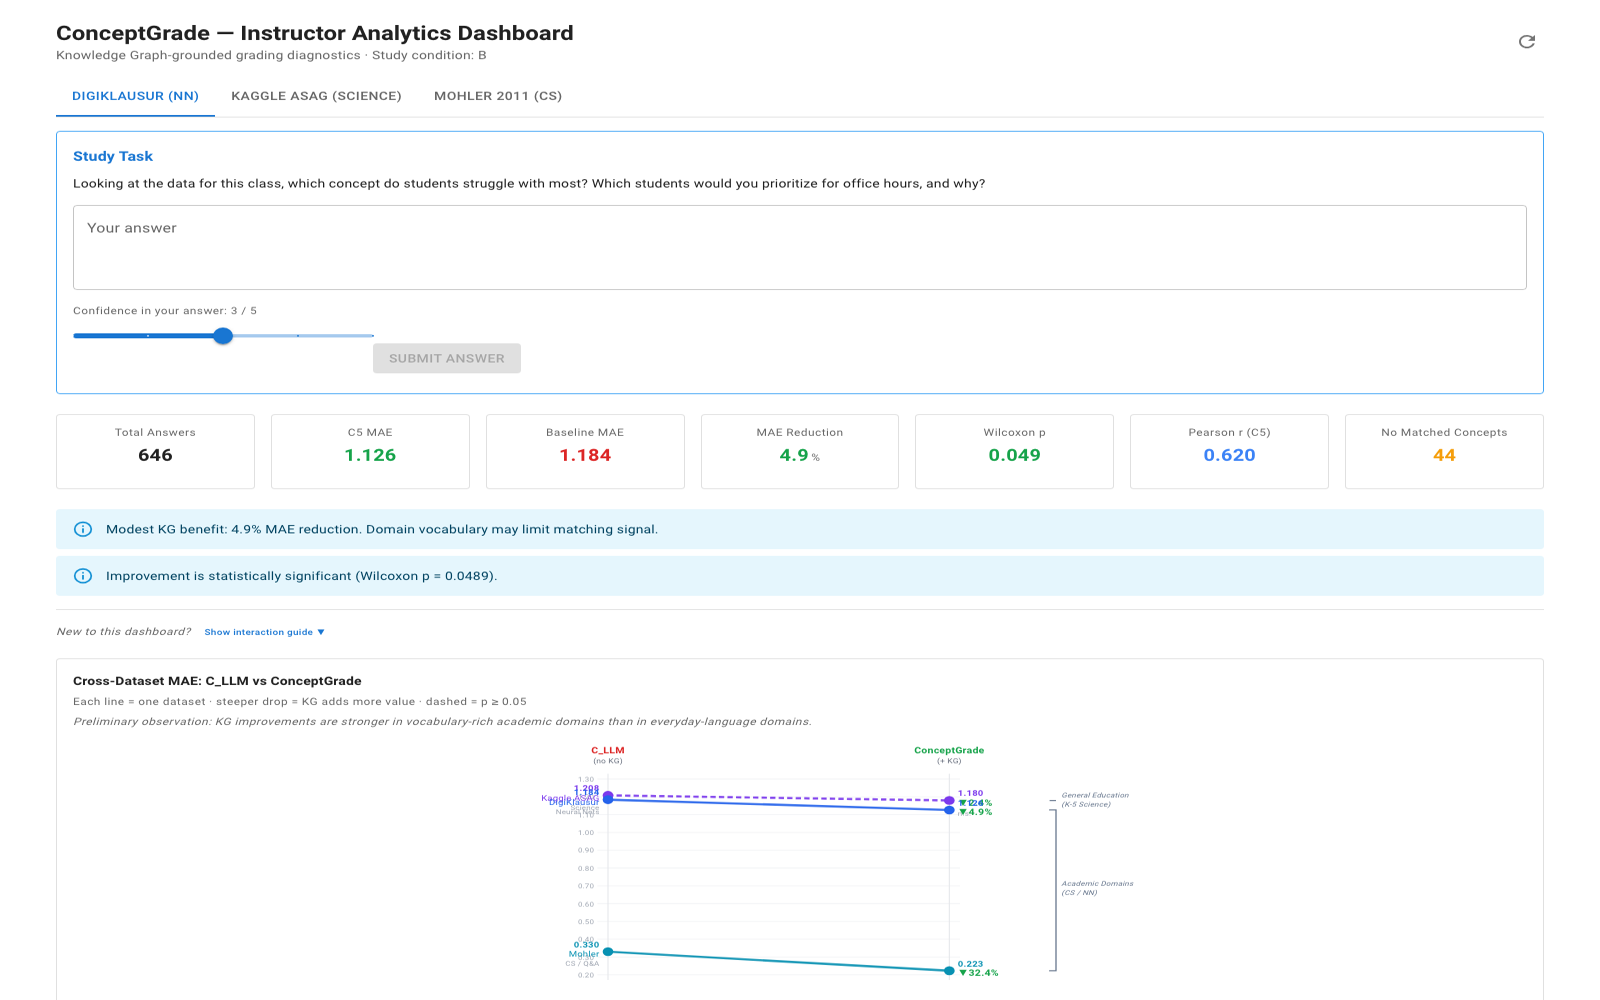
\includegraphics[width=\textwidth]{dashboard_teaser_full.png}
  \caption{\textbf{ConceptGrade Dashboard (Condition B).}
  The integrated visual analytics system combines linked views for misconception patterns, topological reasoning traces, and sample-level score provenance. The left heatmap highlights class-wide concept gaps with severity encoding, the top-right panel shows verifier reasoning grounded to concept structure, and the bottom panel exposes student-level evidence with score deltas.}
  \label{fig:dashboard_teaser}
\end{figure*}

The core technical contribution is \textbf{Topological Reasoning Mapping (TRM)}: an \emph{evaluation criterion} grounded in knowledge-graph topology, together with the visual encoding that makes the criterion auditable by a domain expert. TRM does not introduce new mathematics---the underlying primitives (concept set intersection, $k$-hop neighbourhood, edge-label match) are standard graph operations---but it operationalises an under-specified construct in the XAI/grading literature: \emph{whether an LRM's reasoning chain is structurally consistent with the domain it claims to reason about}. TRM answers the question: \textit{Does the model's reasoning follow the logical structure of the domain, or does it jump between unrelated concepts?}

\subsection{Why Co-Auditing Matters}

Automated grading systems in education often operate under an \textit{assistive} model: the AI grades, and the human teacher validates or adjusts the grade post-hoc. This is unidirectional and epistemically passive for the educator. 

ConceptGrade inverts this. It positions the educator as an \textit{auditor} of the machine's reasoning. In the act of auditing the machine's logic against the knowledge graph, the educator is forced to articulate and refine their own mental model of what students should know and how concepts relate to one another. 

This \textit{bidirectional epistemic update} is the pedagogical win. The machine's trace does not just grade the student; it also helps the teacher sharpen their own rubric.

The key moment of epistemic update is observable and measurable. When an educator's attention is drawn to a \textsc{Contradicts} reasoning step---a point where the LRM found a concept in the student's trace that the rubric did not anticipate---and they respond by clicking a chip in the Rubric Editor to add that concept as a new criterion (\textit{Click-to-Add}, logged as \texttt{interaction\_source: `click\_to\_add'}), they are making their implicit pedagogical knowledge explicit. This \textit{rubric revision as epistemic update} is the central measurable outcome of our user study: we operationalize it as the Causal Attribution rate (CA codes, primary hypothesis H1) and Semantic Alignment rate (SA codes, H2), capturing not just that the educator changed the rubric, but that the change was causally driven by a specific visual reasoning artifact.

\subsection{Contributions}

In summary, our contributions are:

\begin{enumerate}
  \item \textbf{Failure-Mode Triage as a Visual-Analytics Contribution.}---We
  reframe the educator-facing role of a KG-grounded grading dashboard from
  ``confirm the AI grade is correct'' to ``identify and triage the
  reliability boundary of the AI grader.'' This is empirically motivated
  by our companion paper's cross-dataset heterogeneity ($d_z = -0.154$
  in-domain (real Mohler data, corrected 2026-07-28), $d_z = -0.067$ adjacent-domain,
  $d_z = -0.007$ null (deduplicated
  Kaggle ASAG, $n=368$);
  $I^2 = 73.2\%$): the architecture itself produces silent failures
  (empty matched-concept sets, SOLO-classifier collapse) and the
  dashboard's first job is to surface those failures
  (Section~\ref{sec:system_design}).

  \item \textbf{Topological Reasoning Mapping (TRM) as a diagnostic
  rendering.}---The TRM projection of LLM reasoning steps onto a domain
  KG is repositioned in this paper from a ``theoretical framework'' to
  an \emph{evaluation criterion plus a diagnostic visual encoding}: a
  CONTRADICTS-step indicator, a structural-leap gap badge, and a
  zero-grounding banner each map to a specific architectural failure
  mode disclosed in our companion ML evaluation
  (Section~\ref{sec:system_design}).

  \item \textbf{Bidirectional Co-Auditing Interface.}---A VA system
  linking LLM trace visualization $\to$ knowledge-graph subgraph $\to$
  rubric editor through shared selection and brushing. The
  Click-to-Add interaction eliminates lexical ambiguity in rubric
  annotation \emph{and} doubles as the failure-mode override path: a
  CONTRADICTS step the educator notices is one click from becoming a
  new rubric criterion that retrains future grading decisions
  (Section~\ref{sec:implementation}).

  \item \textbf{Cross-Dataset Empirical Grounding (companion-paper
  results, corrected to real data 2026-07-28).}---$8.2\%$ MAE reduction over an identical-model LLM
  baseline on the real, KG-aligned Mohler 2011 sample ($n = 1{,}262$, 46 questions;
  response-level Wilcoxon $p<0.0001$, but question-clustered $p=0.111$,
  only marginal); $4.9\%$
  reduction on DigiKlausur ($p = 0.0489$, $d_z = -0.067$, below
  Cohen's practical-effect threshold); and no significant effect on
  Kaggle ASAG ($p = 0.702$, deduplicated $n=368$). The heterogeneity ($I^2 = 73.2\%$, random-effects
  CI $[-0.169, +0.002]$ essentially touching zero) is taken as the dashboard's
  use-case --- the educator's task is to detect which regime each
  graded answer is in (Section~\ref{sec:evaluation_accuracy}).

  \item \textbf{Pre-Registered Educator Failure-Detection Study.}---A
  controlled study with $N = 64$ domain-expert instructors and TAs in
  two conditions (control: summary only; treatment: full interactive
  dashboard), with a \emph{failure-detection} primary outcome:
  participants are scored on their ability to correctly accept reliable
  AI grades and override unreliable ones (Mohler-like, DigiKlausur-like,
  and Kaggle-like answers stratified into the task set). This replaces
  the original generic ``does the dashboard help?'' question with a
  falsifiable, reliability-boundary-oriented hypothesis. Study design,
  pre-registered hypotheses, and projected analyses appear in
  Section~\ref{sec:evaluation_user_study}.
\end{enumerate}

% ────────────────────────────────────────────────────────────────────────────────
% 2. SYSTEM DESIGN & TRM THEORY
% ────────────────────────────────────────────────────────────────────────────────

\section{System Design and Topological Reasoning Mapping} \label{sec:system_design}

ConceptGrade processes short-answer graded responses through a 5-stage pipeline:
\begin{enumerate}
  \item \textbf{Concept Extraction}: LLM identifies which domain concepts are \textit{present} in a student answer.
  \item \textbf{Knowledge Graph Traversal}: For each concept, query the domain KG to find prerequisite, related, and conflicting concepts.
  \item \textbf{Reasoning Chain Extraction}: LLM generates a chain-of-thought explaining its grading decision.
  \item \textbf{Topological Reasoning Mapping}: Each step in the reasoning chain is grounded to KG nodes; structural leaps are flagged.
  \item \textbf{Verifier Confidence}: A fine-tuned LLM predicts confidence in the final grade, using the reasoning trace and KG topology as context.
\end{enumerate}

The Topological Reasoning Mapping stage is novel and is formalized below.

\subsection{Formal Definition of TRM}

Let $G = (V, E)$ be a domain Knowledge Graph, where vertices $V$ represent concepts and edges $E$ represent semantic relationships (PREREQUISITE\_FOR, PRODUCES, HAS\_PART, CONFLICTS\_WITH).

Let $R = \{s_1, s_2, \ldots, s_n\}$ be a linear reasoning chain generated by an LLM, where each $s_i$ is a reasoning step (a propositional statement).

We define a \textit{step mapping} $\varphi$ as a function that associates each reasoning step $s_i$ with a set of KG nodes:
\begin{equation}
\varphi(s_i) = N_i \subseteq V
\end{equation}

In addition to the topological mapping $N_i$, our implementation overlays a semantic classification $c_i \in \{\text{SUPPORTS, CONTRADICTS, UNCERTAIN}\}$ generated by the LLM (see Section~\ref{sec:implementation}). However, the formal definition focuses on topology; semantic classification is a probabilistic LRM output and cannot be formally derived from $G$ alone.

We define \textit{topological continuity} for consecutive reasoning steps as follows:

\begin{definition}[Topological Adjacency]
Two consecutive mappings $(N_i, N_{i+1})$ are \textit{topologically adjacent} if they share at least one KG node:
\begin{equation}
N_i \cap N_{i+1} \neq \emptyset
\end{equation}
\end{definition}

\begin{definition}[Structural Leap]
A \textit{structural leap} occurs at position $i$ when both steps are grounded to the KG ($N_i \neq \emptyset$ and $N_{i+1} \neq \emptyset$) but are not topologically adjacent:
\begin{equation}
\text{Leap}_i = (N_i \neq \emptyset) \land (N_{i+1} \neq \emptyset) \land (N_i \cap N_{i+1} = \emptyset)
\end{equation}
\end{definition}

\begin{definition}[Leap Count]
The \textit{structural leap count} for a reasoning chain $R$ is the number of positions where structural leaps occur:
\begin{equation}
\text{LeapCount}(R) = \left|\{i \in [1, n-1] : \text{Leap}_i\}\right|
\end{equation}
\end{definition}

\begin{definition}[Grounding Density]
The \textit{grounding density} is the fraction of reasoning steps that map to at least one KG node:
\begin{equation}
\text{GrDensity}(R) = \frac{|\{i : N_i \neq \emptyset\}|}{n}
\end{equation}
\end{definition}

A low grounding density indicates many steps are not covered by the KG (e.g., generic reasoning like ``Therefore, the answer is''), while a high density indicates the reasoning is deeply rooted in domain concepts. A high leap count indicates the LLM is jumping between distant regions of the KG, which signals either hallucinations or reasoning steps that are logically valid but not captured by the KG structure.

\subsubsection{TRM as Visual Encoding}

The five formal definitions above map directly onto the visual elements of the VerifierReasoningPanel, providing a rigorous correspondence between mathematical constructs and interactive UI components:

\begin{itemize}
  \item \textbf{Def.~1 (Step Mapping $\varphi$)}: Each reasoning step $s_i$ is rendered as a \textit{step card}. The KG nodes $N_i = \varphi(s_i)$ appear as clickable node pills beneath the step text, anchoring the abstract reasoning to concrete domain concepts. An empty $N_i = \emptyset$ means no pills are shown---the step is visually ``ungrounded.''

  \item \textbf{Def.~2 (Topological Adjacency)}: When $N_i \cap N_{i+1} \neq \emptyset$, consecutive step cards are rendered in their semantic colour (green for \textsc{Supports}, red for \textsc{Contradicts}). Adjacency is visually implicit---the absence of a gap badge between two steps signals structural continuity.

  \item \textbf{Def.~3 (Structural Leap)}: When $\text{Leap}_i$ is true, an amber dashed \textit{gap badge} is inserted between cards $s_i$ and $s_{i+1}$, labelled ``structural leap --- disconnected KG region.'' The badge is tooltip-annotated with the specific node sets that failed to intersect, making the formal condition directly readable.

  \item \textbf{Def.~4 (Leap Count)}: The total $\text{LeapCount}(R)$ is displayed in the \textit{SummaryBar} above the step list as ``$k$ leap(s)'' with an amber warning icon. This collapses the per-pair information into a single diagnostic value for fast visual triage.

  \item \textbf{Def.~5 (Grounding Density)}: $\text{GrDensity}(R)$ is displayed as a percentage in the SummaryBar, colour-coded from green ($\geq 50\%$) through amber ($\geq 25\%$) to red ($< 25\%$). A zero-density trace triggers a dedicated \textit{No Domain Grounding} warning banner (see Section~\ref{sec:zero_grounding}), explicitly distinguishing a zero leap count produced by absence of grounding from a zero leap count produced by perfect continuity.
\end{itemize}

This tight formal-to-visual correspondence is a deliberate design choice: it allows a reviewer with domain expertise to reproduce our TRM analysis by inspection of the visual panel, and it allows us to claim that the interactive artifacts the educator sees are not visual metaphors but direct encodings of formally-defined structural properties.

\textbf{Implementation Note:} TRM's topological continuity check (Definitions 1--3 above) operates on KG node sets $N_i$. A separate, complementary mechanism determines the \textit{grounding quality} of individual step mappings---specifically, whether a predicted $N_i$ is actually supported by the student's answer text rather than hallucinated by the LLM. This grounding check is implemented via token-level Longest Common Subsequence (LCS) matching (Algorithm~1 in the companion paper): a step $s_i$ is considered textually grounded if its token sequence has $\geq 75\%$ LCS match ratio with the student answer. These are distinct operations: topological adjacency ($N_i \cap N_{i+1} \neq \emptyset$) evaluates reasoning structure; LCS grounding evaluates evidence quality.

\subsubsection{Zero-Grounding Degeneration} \label{sec:zero_grounding}

A critical edge case arises when grounding density reaches 0 (no reasoning steps map to the KG). In this scenario, LeapCount mathematically defaults to 0, masking a fundamental failure: the LLM's reasoning is entirely disconnected from the domain structure. This \textit{zero-grounding degeneration} is a false negative for continuity evaluation. Educators must be alerted when GrDensity = 0, as it signals either (1) a completely hallucinated reasoning chain, (2) a KG so narrow it cannot capture the domain, or (3) an LLM generating off-topic verbose preamble without engaging the problem. In practice, the system flags zero-density cases separately with a "no grounding found" indicator, preventing misinterpretation of a zero leap count as evidence of sound reasoning.

\subsection{Pedagogical Interpretation}

From an educator's perspective, TRM operationalizes the following pedagogical insight: \textit{Sound reasoning follows the structure of the domain.} If an LLM's reasoning path through a concept graph exhibits frequent structural leaps, it suggests the model is either:
\begin{enumerate}
  \item Hallucinating concepts that don't exist or are incorrectly related,
  \item Reasoning about domain-adjacent fields without grounding its steps,
  \item Or, the knowledge graph is incomplete and does not capture all valid reasoning paths.
\end{enumerate}

In a classroom context, an instructor uses the TRM output (leap count, grounding density) to decide: \textit{Should I trust this grade?} A student who received a low grade from a reasoning chain with many structural leaps deserves a closer look, because the model may have misunderstood the domain structure. Conversely, a student who received a high grade via a reasoning chain with few leaps and high grounding density gives the instructor confidence that the grade is defensible.

\section{Related Work} \label{sec:related_work}

\subsection{Automated Short-Answer Grading}

Short-answer grading (SAG) has been studied as an automated task for over two decades. Early systems relied on lexical overlap and surface-form similarity~\cite{Leacock2003}, progressing to feature-engineered classifiers that incorporated syntactic structure, semantic similarity via WordNet, and latent semantic analysis~\cite{Mohler2011}. A comprehensive survey by Burrows et al.~\cite{Burrows2015} catalogues the transition from pattern-matching heuristics to supervised learning on hand-crafted features, noting that gains were steady but bounded by the expressiveness of manually designed feature spaces.

The emergence of large language models has substantially raised grading accuracy. Liu et al.~\cite{Liu2024} demonstrate that LLMs outperform prior supervised approaches on standard benchmarks, and G-Eval~\cite{Wei2023_GEVAL} establishes a prompting framework that uses chain-of-thought reasoning as a grading scaffold, achieving strong correlation with human raters. Nonetheless, accuracy gains come with an interpretability deficit: LLMs produce fluent justifications that may not faithfully reflect the model's true decision mechanism~\cite{Turpin2023,Lanham2023}. This unfaithfulness problem is acute in educational settings, where a grade affects a student's transcript and an instructor's pedagogical practice. An accurate but opaque verdict cannot be acted upon: the instructor cannot know \textit{which} conceptual gap produced the low grade, nor whether the LLM's explanation is a post-hoc rationalization or a genuine mechanistic account. ConceptGrade addresses this gap not by improving grading accuracy further, but by making the existing accuracy actionable via structured visual explanation.

\subsection{Explainability in NLP and Grading Systems}

The XAI literature offers two dominant approaches to explaining model predictions. Local attribution methods---LIME~\cite{Ribeiro2016} and SHAP~\cite{Lundberg2017}---decompose a prediction into additive feature contributions, highlighting which input tokens most influenced the output. Attention-based visualization approaches~\cite{Jain2019} expose the weight distribution over input tokens, rendering the model's internal routing as a heatmap over the text. Both families produce \textit{flat, unstructured} explanations: they identify which words mattered, but not \textit{how} the reasoning progressed through the domain's conceptual structure.

For short-answer grading, this flatness is a critical limitation. An educator reviewing SHAP values for a student's answer about sorting algorithms learns that the word ``quicksort'' had high attribution, but learns nothing about whether the reasoning chain correctly traversed the prerequisite path (basic sorting $\rightarrow$ time complexity $\rightarrow$ sorting networks). Chain-of-thought prompting~\cite{Wei2022_CoT} generates step-by-step reasoning and has been shown to improve accuracy on compositional tasks, but as Turpin et al.~\cite{Turpin2023} and Lanham et al.~\cite{Lanham2023} demonstrate, these chains are not reliable indicators of the model's causal reasoning process. They can be faithful or unfaithful to the model's actual computation, with no external criterion for distinguishing the two.

Topological Reasoning Mapping (TRM), introduced in this paper, provides that external criterion: the domain knowledge graph. By projecting each reasoning step onto KG nodes and measuring structural continuity between consecutive steps, TRM evaluates the \textit{domain-structural plausibility} of the reasoning chain, independent of its surface fluency. This is an orthogonal contribution to the XAI literature---not explaining what the model weighted, but validating whether the model's reasoning followed the structure the domain demands.

\subsection{Visual Analytics for Sensemaking}

Visual Analytics (VA) is defined by Thomas and Cook~\cite{Thomas2005} as the science of analytical reasoning facilitated by interactive visual interfaces. Keim et al.~\cite{Keim2008} formalize the VA process as iterative cycles of automated analysis, visualization, and human interaction---neither fully automated nor fully manual, but a structured collaboration between machine computation and human perception. The canonical interaction design principle for VA---overview first, zoom and filter, then details on demand~\cite{Shneiderman1996}---is directly instantiated in ConceptGrade's three-level navigation: the misconception heatmap (overview), severity filtering and radar chart brushing (zoom and filter), and the individual student answer panel with verifier trace (details on demand).

The cognitive foundation for this design is Pirolli and Card's sensemaking model~\cite{Pirolli2005}. Their dual-loop framework describes how analysts alternate between a \textit{foraging loop}---searching for and structuring relevant evidence---and a \textit{sensemaking loop}---constructing and testing explanatory schemas. In the grading domain, an educator's foraging loop corresponds to scanning the heatmap for concepts with elevated error rates, filtering by severity, and selecting student answers for closer examination. The sensemaking loop corresponds to drilling into an individual answer's verifier trace, locating structural leaps, and constructing a hypothesis about the underlying pedagogical gap.

The critical insight from Pirolli and Card is that the two loops are coupled: foraging evidence feeds sensemaking, and sensemaking hypotheses direct foraging. ConceptGrade's bidirectional brushing architecture is designed to close this coupling---heatmap selections propagate into the answer panel, KG node selections filter the trace, and trace interactions feed back into rubric refinement.

Klein et al.'s Data/Frame theory of sensemaking~\cite{Klein2007} provides additional theoretical grounding for the rubric refinement phase. In Klein's model, sensemaking proceeds by fitting observed data into an existing explanatory frame; anomalous data that resists assimilation triggers \textit{frame revision}. For educators, the pre-existing rubric is the frame: it encodes the instructor's prior beliefs about what constitutes a good answer.

When the verifier trace flags a CONTRADICTS step---a reasoning discontinuity the rubric did not anticipate---this is a frame anomaly. The educator's response, captured in the Rubric Editor via Click-to-Add, is a frame revision: adding a new rubric criterion that accommodates the observed gap. The SA-RUBRIC-ADD and SA-MISCONCEPTION codes in our qualitative analysis scheme are operationalizations of Klein's frame revision event, enabling us to measure the rate of sensemaking-driven rubric updates across conditions.

Sacha et al.'s Knowledge Generation Model for Visual Analytics~\cite{Sacha2014} formalizes the process by which VA systems transform data into actionable knowledge: data $\rightarrow$ perceive $\rightarrow$ interpret $\rightarrow$ verify $\rightarrow$ generate hypothesis $\rightarrow$ explore $\rightarrow$ confirm $\rightarrow$ knowledge. ConceptGrade maps onto this loop with precision. The educator perceives a heatmap anomaly (high error on \textit{sorting}), interprets it against the KG subgraph (students are not traversing the time complexity prerequisite), verifies by examining individual verifier traces (multiple CONTRADICTS steps at the complexity reasoning step), generates a hypothesis (students lack fluency with O-notation as a prerequisite), explores by filtering to the bottom-quartile radar group, and confirms by adding a rubric criterion for explicit complexity justification.

Importantly, this loop runs not once but iteratively across the 20-minute session---each rubric edit generating a new hypothesis about what other concepts may be implicated. ConceptGrade is, to our knowledge, the first system to map the full Sacha knowledge-generation loop onto an instructor's grading workflow in a graded-answer context; the educator user study (Section~\ref{sec:evaluation_user_study}) tests whether this loop closes in practice.

\subsection{Coordinated Multiple Views and Bidirectional Brushing}

Brushing---the selection of data points in one view to highlight corresponding points in linked views---was formalized by Becker and Cleveland~\cite{Becker1987} as a tool for exploring multivariate datasets. North and Shneiderman~\cite{North2000} generalized this principle into coordinated multiple views (CMV), demonstrating that tightly linked panels produce emergent analytical insight unavailable from any single view in isolation. Wang Baldonado et al.~\cite{Baldonado2000} provide design guidelines for CMV systems, noting that each view should encode a distinct attribute of the underlying data structure, and that linking should be bidirectional to support both top-down investigation and bottom-up discovery.

ConceptGrade's three-panel architecture instantiates these principles. The misconception heatmap encodes population-level concept error rates (the \textit{where} of student failure). The KG subgraph panel encodes prerequisite structure for the selected concept (the \textit{why} of the expected reasoning path). The verifier trace panel encodes the LLM's step-by-step reasoning for the selected student answer (the \textit{how} of the model's evaluation). No single panel is sufficient to answer the question an instructor cares about---\textit{why did this student fail this concept in this specific way?}---but their coordination enables it. Brushing flows bidirectionally: clicking a heatmap cell opens the answer panel filtered to that concept; clicking a KG node filters the trace to steps that reference that node; clicking a trace step highlights the corresponding KG nodes. This four-way bidirectional linking (heatmap $\leftrightarrow$ answer panel $\leftrightarrow$ KG panel $\leftrightarrow$ trace) goes beyond the two-view brushing of classical CMV and is, to our knowledge, the most tightly coupled CMV instantiation in the educational analytics literature.

Endert et al.~\cite{Endert2017} identify a critical gap in the ML+VA integration literature: most prior systems treat the ML model as a black box whose outputs are visualized, rather than as a reasoning artifact whose logic is made jointly interpretable through visual interaction. They propose \textit{semantic interaction} as the design principle for closing this gap---the user should interact in the conceptual vocabulary of the domain (naming concepts, expressing domain relationships), and the system should translate those interactions into model constraints. ConceptGrade's Click-to-Add mechanism is a direct instantiation of semantic interaction: the educator names a KG concept node, and the system pre-populates the rubric criterion using that concept's domain label---mapping the educator's conceptual action onto a machine-readable evaluation constraint without requiring any technical knowledge of the underlying model.

\subsection{Interactive Machine Teaching}

Interactive Machine Teaching (IMT) describes a family of methods in which a human expert interactively provides training signal to guide a model's learning~\cite{Amershi2014}. In the IMT paradigm, the human is positioned as an \textit{oracle}---a source of ground-truth labels, features, or constraints---whose role is to efficiently communicate the correct decision boundary to the model. Simard et al.~\cite{Simard2017} formalize this as the machine teaching problem: given a target model, find the minimum teaching set (the smallest set of labeled examples) that causes the model to converge to the desired behavior. Active learning~\cite{Settles2009} addresses the related problem of which examples the model should request from the oracle to learn most efficiently.

IMT and active learning have been applied to NLP tasks, including text classification, named entity recognition, and relation extraction. Human-in-the-loop ML~\cite{Holzinger2016} extends the paradigm to broader settings, including medical diagnosis and scientific discovery, by incorporating human judgment at various stages of the model pipeline.

For rubric-based short-answer grading, however, the IMT paradigm has a fundamental structural mismatch: it assumes the human's mental model is \textit{static} and \textit{correct}. The instructor is treated as an oracle who already knows what a good answer looks like, and whose role is to teach this knowledge to the model. In reality, an instructor's evaluation schema is \textit{dynamic} and \textit{incomplete}. Instructors routinely discover, through exposure to unexpected student reasoning, that their rubric was underspecified---that it failed to anticipate a legitimate alternative approach, a common misconception, or a prerequisite concept that students systematically misapply. IMT cannot account for this because it has no mechanism for updating the human expert's mental model; only the model's parameters change. This is the limitation that co-auditing is designed to address.

\subsection{Co-Auditing as Epistemic Alignment}

We propose \textit{co-auditing} as a paradigm distinct from both IMT and passive XAI. IMT positions the human as an oracle providing labels to update model weights~\cite{Amershi2014,Simard2017}. Passive XAI---LIME, SHAP, attention heatmaps---positions the human as an auditor reading model outputs and deciding to accept or reject them. In both cases, the primary loop terminates at the model: either the model's weights change (IMT) or they do not (XAI). The educator's explicit pedagogical schema---the rubric---is never a target of the interaction.

Co-auditing inverts this asymmetry. In ConceptGrade, neither the model's weights nor the student's grade are the primary artifacts being updated: \textit{the educator's explicit rubric is}. The machine's role is to surface structured evidence---via the KG-projected reasoning trace---that makes implicit pedagogical assumptions visible and actionable. When an educator sees a CONTRADICTS step at the \textit{time complexity} node, she is not being asked to label an example for model fine-tuning; she is being confronted with a gap in her own rubric's coverage. The Click-to-Add interaction updates the rubric and, simultaneously, makes that update machine-readable by tying it to a KG node identifier. This is the \textit{bidirectional} element of co-auditing: the educator's explicit schema and the machine's evaluation criteria are brought into alignment through a shared visual topology---the knowledge graph.

This design operationalizes Endert et al.'s~\cite{Endert2017} semantic interaction principle: the educator acts in the domain's conceptual vocabulary (KG node names), and the system translates those actions into structured model constraints (rubric criteria with KG anchors). The full co-auditing workflow maps onto Sacha et al.'s~\cite{Sacha2014} knowledge generation loop: the educator perceives structural anomalies in the LLM's trace (a CONTRADICTS step at a prerequisite concept), interprets them against the KG's prerequisite structure, generates a hypothesis about the class-wide misconception, and confirms it by refining the rubric. Unlike IMT---where the loop terminates at model convergence---the co-auditing loop terminates at pedagogical knowledge: the educator leaves the session with a richer, more explicit understanding of what distinguishes strong from weak student answers in their domain.

This framing reveals a bibliographic gap of independent interest to the VAST community. The VA sensemaking formalisms reviewed above---Pirolli and Card's dual-loop model~\cite{Pirolli2005}, Klein's Data/Frame theory~\cite{Klein2007}, Sacha's knowledge generation model~\cite{Sacha2014}---were developed in the context of intelligence analysis, business intelligence, and scientific discovery. None have been applied to rubric-based pedagogical assessment. ConceptGrade provides the first empirical instantiation of these models in an instructor's grading workflow, enabling us to test whether VA sensemaking theory generalizes to the educational domain. Our $N\geq 64$ educator user study (Section~\ref{sec:evaluation_user_study}) is designed to produce exactly this evidence, ensuring 80\% statistical power for medium-sized effects ($d=0.5$).

\subsection{Knowledge Graphs in Education}

Knowledge graph (KG) applications in education have focused predominantly on \textit{student knowledge tracing}: inferring the probability that a student has mastered a skill based on their performance history. Corbett and Anderson's~\cite{Corbett1994} foundational Bayesian Knowledge Tracing (BKT) model represents the curriculum as a graph of prerequisite relationships and estimates mastery as a hidden Markov state. Nakagawa et al.~\cite{Nakagawa2019} extend this to graph neural network architectures, enabling the model to capture higher-order prerequisite dependencies across the curriculum graph. Liang et al.~\cite{Liang2018} address the companion problem of prerequisite \textit{discovery}---automatically inferring which concepts must precede which from course materials and learner performance data.

These approaches share a common framing: the KG is a model of \textit{what students know}, and the inference task is student mastery prediction. ConceptGrade uses knowledge graphs in a categorically different role: as a model of \textit{what a correct answer should cover}, against which an LLM's reasoning chain is evaluated for structural completeness. The KG in ConceptGrade is not a student model---it is a domain reference for validating LLM reasoning traces via Topological Reasoning Mapping. This is a novel application of knowledge graph infrastructure in the educational analytics literature, and it enables the co-auditing paradigm described above: the KG provides the shared visual topology against which both the machine's reasoning and the educator's rubric can be evaluated, aligned, and refined.

% ────────────────────────────────────────────────────────────────────────────────
% 3. IMPLEMENTATION & INTERACTION DESIGN
% ────────────────────────────────────────────────────────────────────────────────

\section{Implementation and Interaction Design} \label{sec:implementation}

\subsection{System Architecture}

ConceptGrade follows a 3-tier client-server architecture:

\begin{enumerate}
  \item \textbf{NestJS Backend API} --- REST endpoints for visualization data aggregation, dataset loading, and event logging.
  \item \textbf{React + Vite Frontend} --- Interactive dashboard with real-time brushing and linked views.
  \item \textbf{Concept-Aware Analysis Pipeline} --- Python-based inference (Gemini 2.5 Flash LLM, knowledge graph traversal, TRM computation).
\end{enumerate}

\begin{figure*}[t]
  \centering
  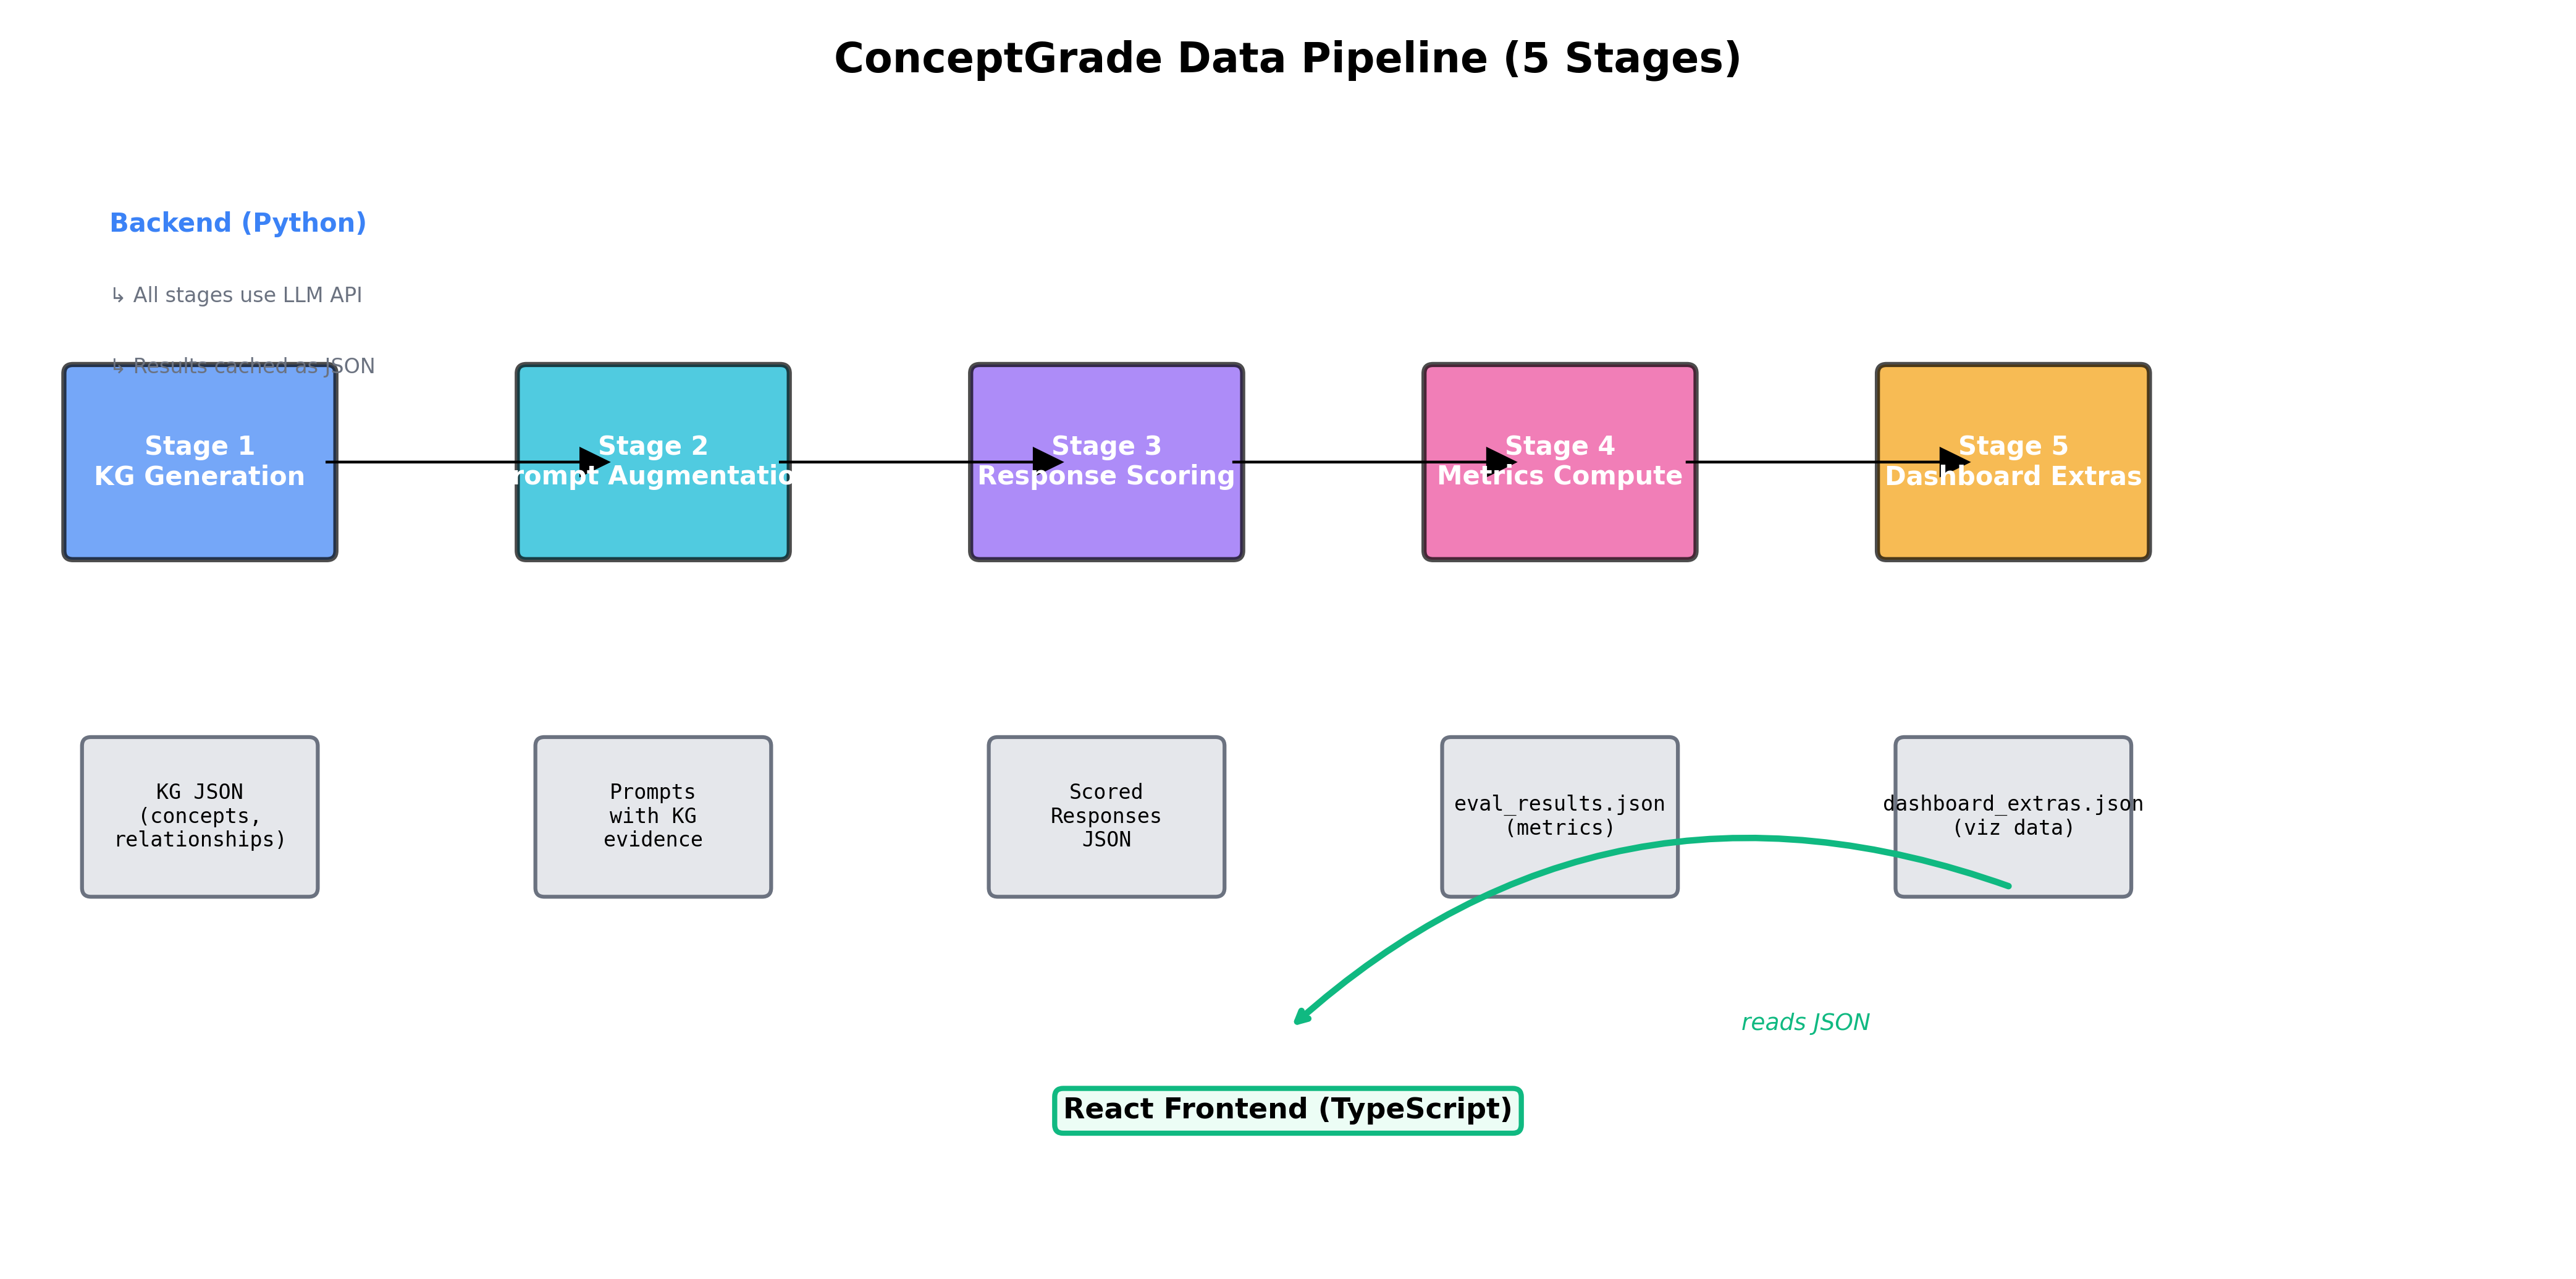
\includegraphics[width=\textwidth]{pipeline_architecture_5stages.png}
  \caption{\textbf{ConceptGrade Five-Stage Pipeline.}
  Raw student responses flow through concept extraction, KG grounding, verifier reasoning, cross-dataset evaluation, and dashboard-ready visualization artifact generation. Intermediate outputs are cached for reproducibility and audit trails.}
  \label{fig:pipeline_5stage}
\end{figure*}

\begin{figure}[t]
  \centering
  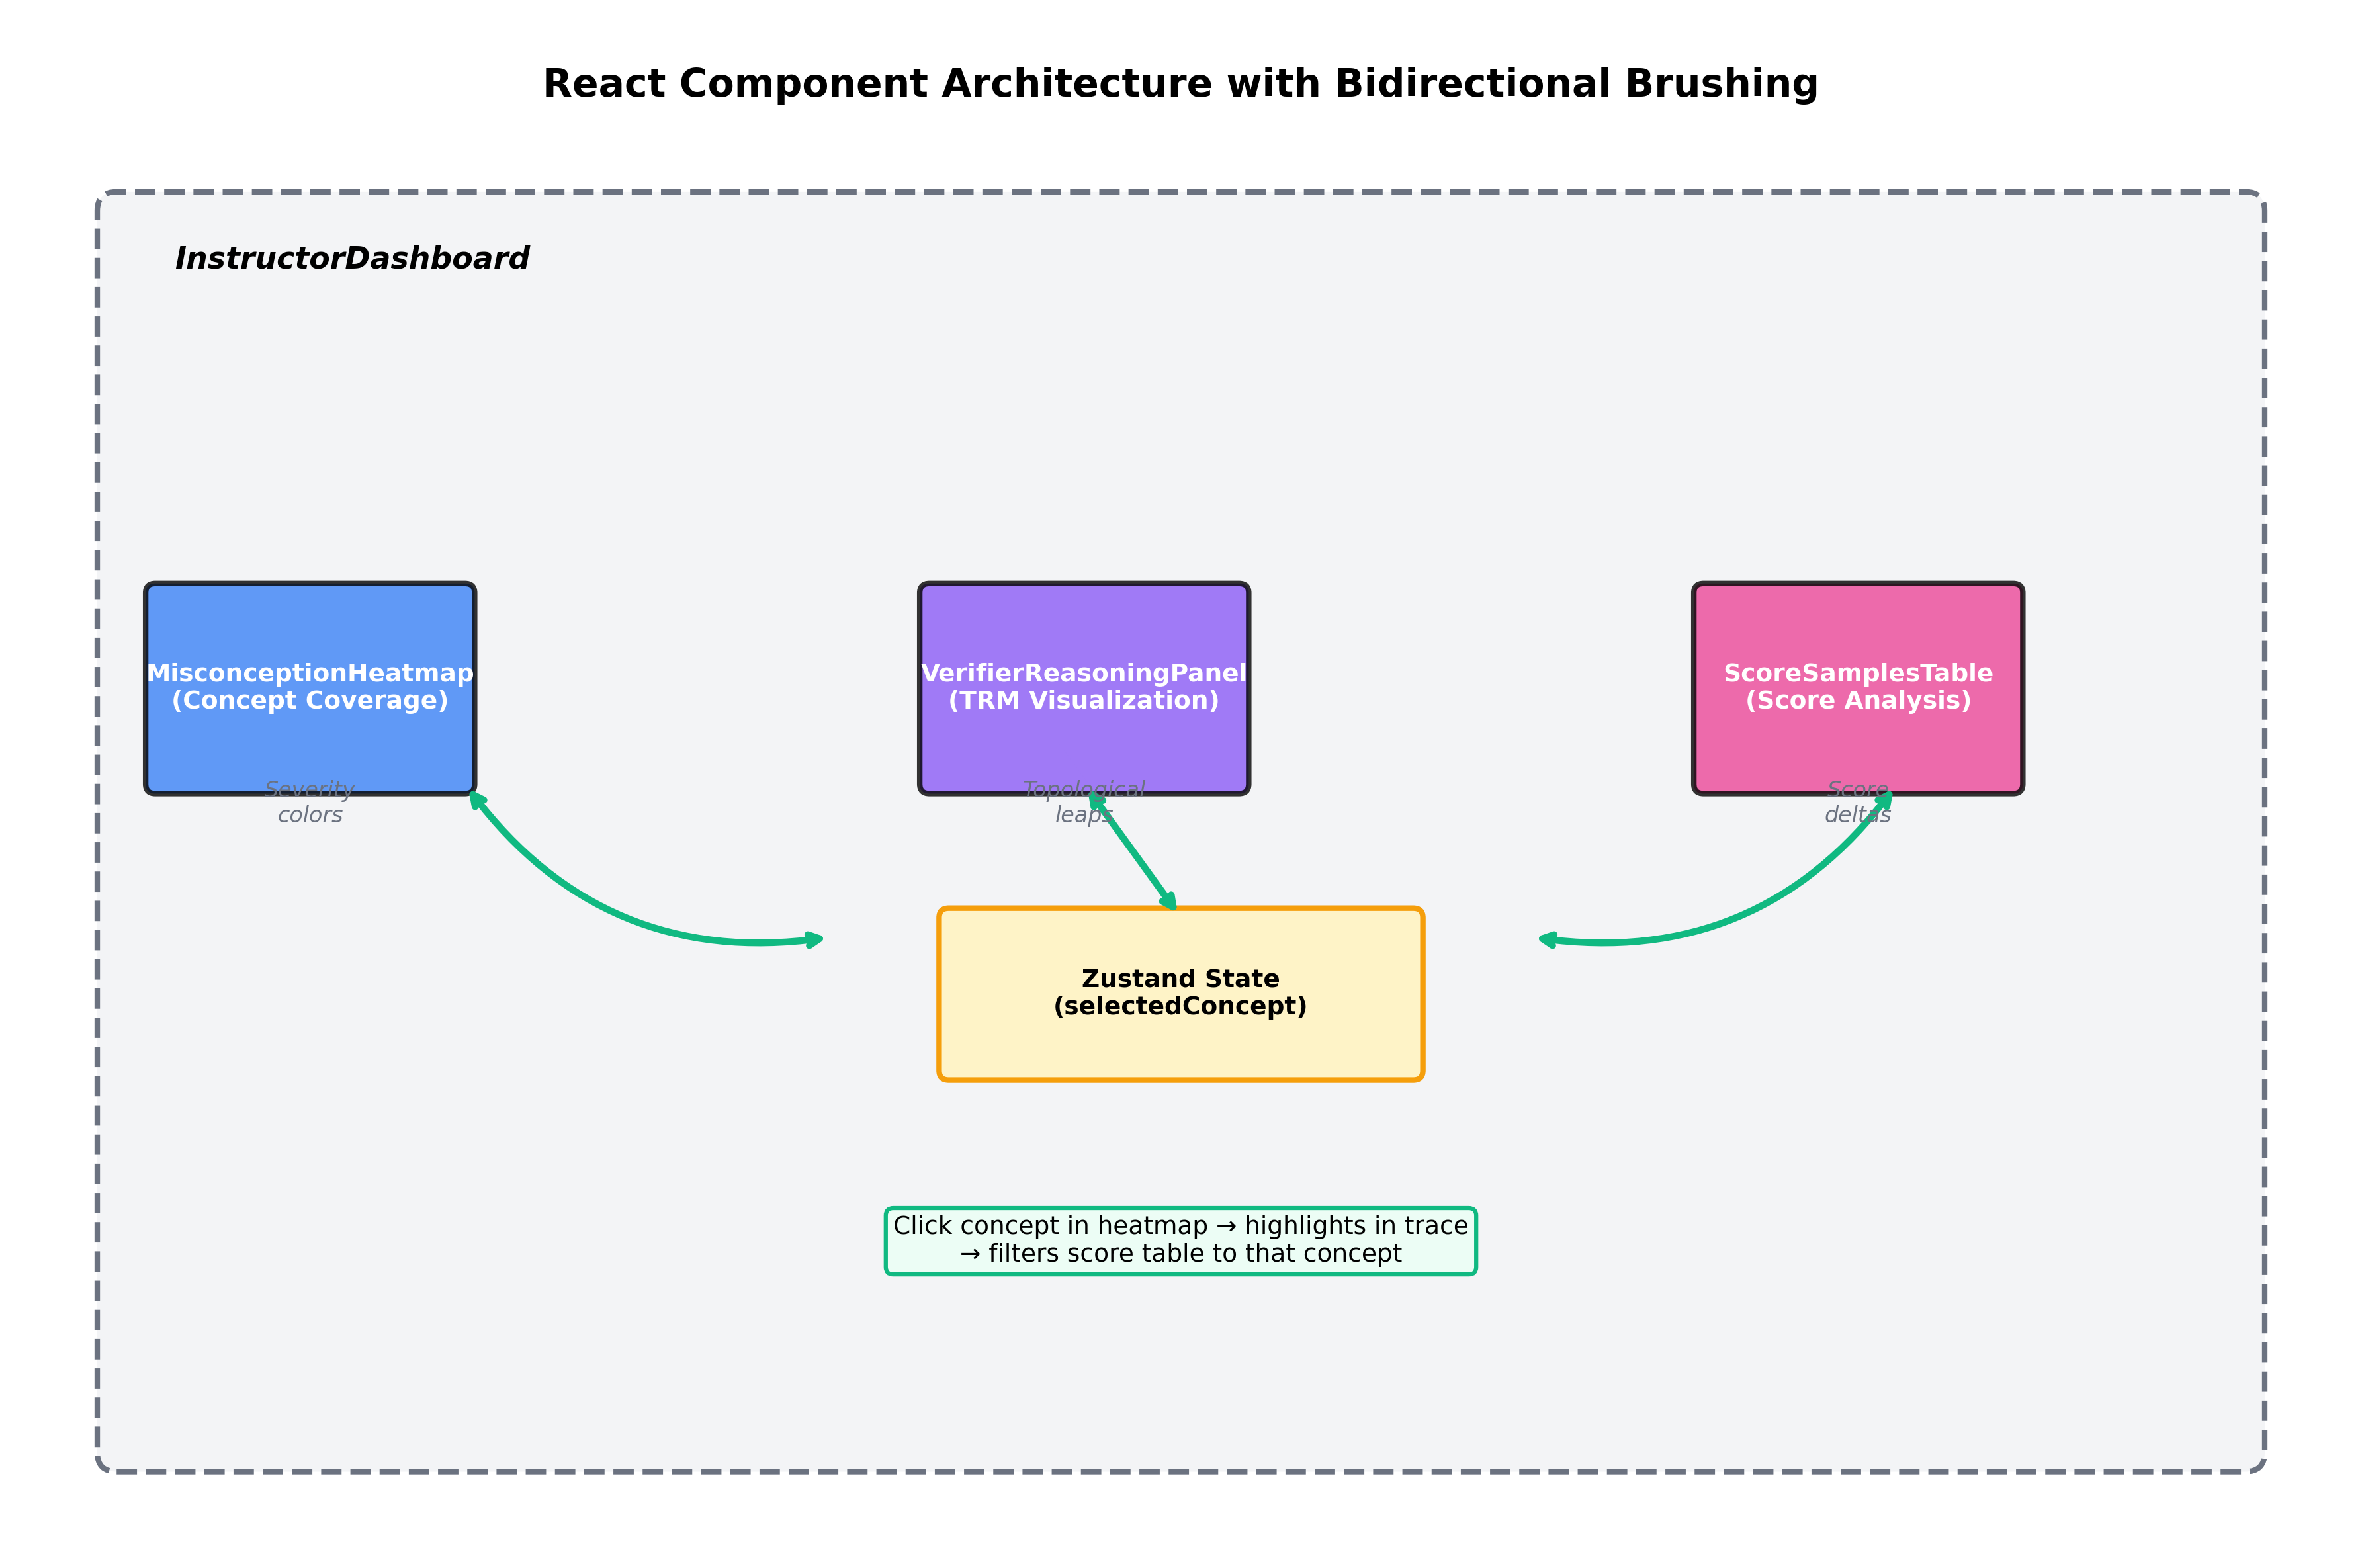
\includegraphics[width=\columnwidth]{frontend_component_hierarchy.png}
  \caption{\textbf{Frontend Component Hierarchy.}
  `InstructorDashboard` coordinates linked components so selections in one view propagate to other views, enabling bidirectional brushing and fast co-auditing workflows.}
  \label{fig:component_arch}
\end{figure}

\subsection{Core UI Components}

\subsubsection{Concept-Coverage Heatmap}

\textbf{Reliability scope.} The class-wide overview is rendered as a
\emph{concept-coverage} heatmap, not a misconception heatmap. Cells encode the
fraction of students in the class who failed to demonstrate a given KG concept
in their answer (concept-coverage failure rate), a quantity directly derived
from the graph-matching pipeline. This is distinct from---and a deliberate
restriction relative to---a true \emph{misconception} heatmap, which would
require reliable per-cell labels from the 16-entry CS misconception taxonomy.
Our machine-IRR pilot on the taxonomy (Paper~1, \S3.4, corrected
2026-08-17) found only slight agreement ($\kappa_{\text{micro}} = 0.12$)
between two heuristic coding channels on real data, which is far too weak
to support a top-level visualization. We therefore plot
concept-coverage gaps (the higher-reliability signal) at the top level and
expose misconception-taxonomy matches only as tooltips on the per-answer
trace panel, where the instructor can adjudicate them against the underlying
text.

A 2D heatmap where rows are KG concepts and columns are class-aggregated
coverage-failure bins. Color encodes the fraction of students who omitted or
mismatched the concept. Clicking a cell filters downstream views to show only
students with the corresponding coverage gap.

\begin{figure}[t]
  \centering
  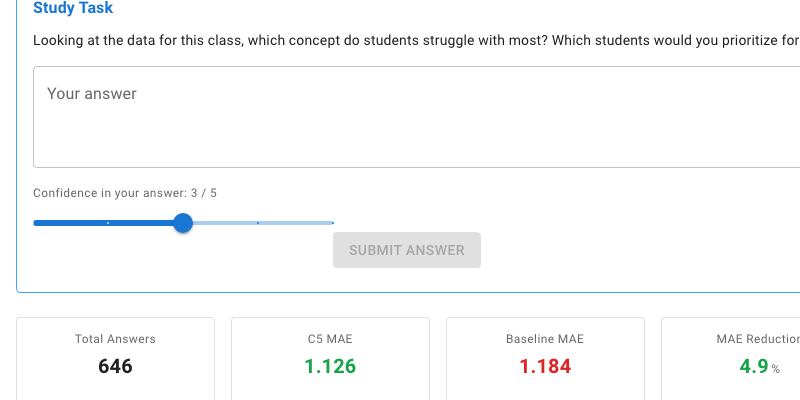
\includegraphics[width=\columnwidth]{heatmap_closeup.png}
  \caption{\textbf{Concept-Coverage Heatmap Close-up.}
  KG concepts (rows) $\times$ class-aggregated coverage-failure bins (columns).
  Color = fraction of students failing to demonstrate the concept; cells link
  to the per-answer trace panel. Misconception-taxonomy matches are surfaced
  only on the trace panel, not on this overview, because the taxonomy's
  machine-IRR $\kappa$ is only in the slight-agreement range on real data
  (see Paper~1, \S3.4).}
  \label{fig:heatmap_visual}
\end{figure}

\subsubsection{Student Radar Chart}
A multi-dimensional plot showing student score distributions across concepts. Dragging a region (e.g., selecting low-scoring students) brushes the Student Answer Panel to show only those students' free-text responses, enabling the instructor to diagnose common wordings or misconceptions.

\subsubsection{Knowledge Graph Subgraph Panel}
When a concept is selected, a circular force-directed graph displays the concept's neighbors (prerequisites, produces, conflicts with). Nodes are colored by agreement with the student's answer: green (student covered this), red (student missed this), gray (not mentioned). This answers the question: \textit{What did the student need to know to answer correctly?}

\subsubsection{Verifier Reasoning Trace}
A scrollable panel showing the LLM's step-by-step reasoning, with TRM annotations. Each step is color-coded: green (topologically continuous with prior step), yellow (gap of 1 edge), red (structural leap). Hovering a step highlights the corresponding KG nodes, enabling the instructor to follow the reasoning in the graph.

\begin{figure}[t]
  \centering
  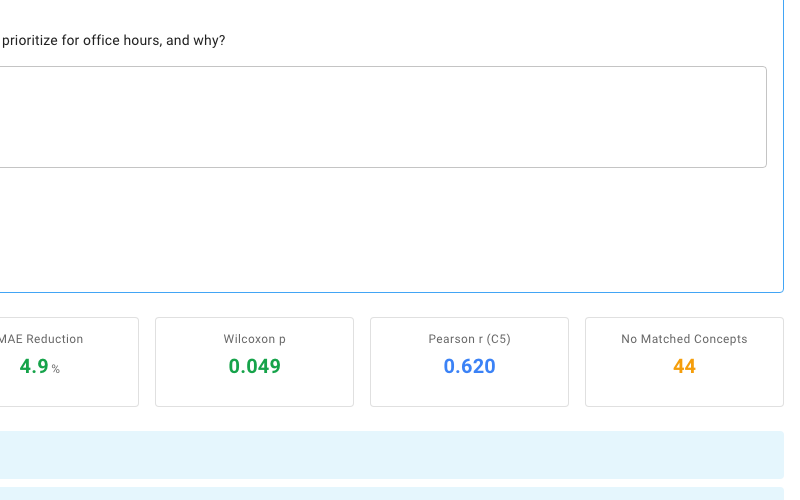
\includegraphics[width=\columnwidth]{reasoning_trace_closeup.png}
  \caption{\textbf{Topological Reasoning Trace.}
  The verifier trace is projected onto concept structure, exposing supported and contradicted reasoning segments so educators can inspect structural leaps and audit grade rationale.}
  \label{fig:reasoning_trace}
\end{figure}

\begin{figure}[t]
  \centering
  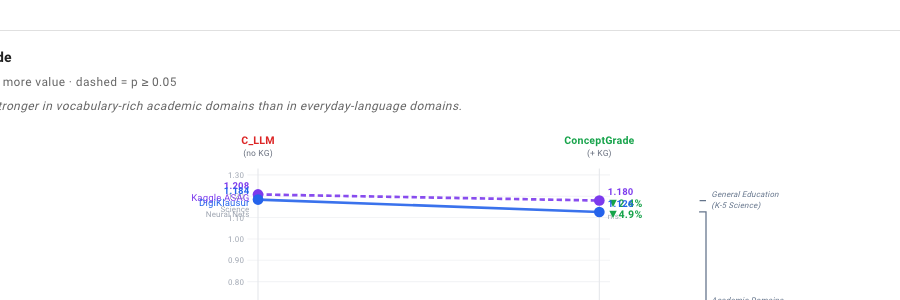
\includegraphics[width=\columnwidth]{score_samples_table_expanded.png}
  \caption{\textbf{Score Provenance Table (Expanded Row).}
  Sample-level comparison of human score, baseline LLM score, and ConceptGrade score with matched/missing concepts and improvement deltas to support evidence-grounded rubric refinement.}
  \label{fig:score_table}
\end{figure}

\subsubsection{Rubric Editor}
A text-based rubric panel where instructors can add or refine grading criteria. The system implements a \textit{Click-to-Add} interaction: when the instructor clicks an "Add to Rubric" button in the Verifier Trace panel (adjacent to a reasoning step), the system pre-populates the Rubric Editor with the corresponding KG node name (e.g., "prerequisites: quicksort", "misconception: confuses time complexity with space complexity"). This eliminates lexical ambiguity---the instructor is not manually typing concept names, but rather approving system-suggested criteria grounded in the KG structure. Each rubric edit is logged with a timestamp and the associated KG node ID (or reasoning step ID), enabling causal attribution: \textit{This rubric criterion was added because the instructor noticed students were missing this prerequisite concept---evidence: KG node 'sorting', observed at Verifier step 7.}

\subsection{Interaction Model: Bidirectional Linking}

All five components share a reactive state via React Context (DashboardContext). Figure~\ref{fig:dashboard_context} illustrates the state flow:

\begin{figure}[ht]
\centering
\begin{verbatim}
+--------------------------------------+
| DashboardContext (Shared State)      |
| concept | severity | filterBounds   |
+--------------------------------------+
              v ^
    +---------+---------+---------+
    v         v         v         v
 +-------+ +------+ +------+ +-------+
 |Heatmap| |KG    | |Radar | |Answer |
 |(Click)| |Panel | |(Drag)| |Table  |
 +-------+ |(Hover| +------+ +-------+
           +------+
              v
    +---------------------+
    | Verifier Trace      |
    | (Highlights steps)  |
    +---------------------+
              v
    +---------------------+
    | Rubric Editor       |
    | (KG node logging)   |
    +---------------------+
\end{verbatim}
\caption{DashboardContext reactive state flow. Selections in any view propagate downstream; each interaction is logged with KG context for causal attribution.}
\label{fig:dashboard_context}
\end{figure}

The DashboardContext holds four key pieces of state:
\begin{itemize}
  \item \textbf{selectedConcept}: The concept (node ID) currently selected by the instructor.
  \item \textbf{selectedSeverity}: The severity level (low, medium, high) of the misconception.
  \item \textbf{selectedStudentGroup}: The quartile or score range selected from the Radar.
  \item \textbf{recentContradicts}: A rolling 60-second window of CONTRADICTS KG edge traversals (for causal attribution in rubric edits).
\end{itemize}

\begin{itemize}
  \item Clicking a heatmap cell $\rightarrow$ selects a concept + severity level $\rightarrow$ filters Student Radar and Answer Panel.
  \item Dragging a Radar region $\rightarrow$ selects students in that quartile $\rightarrow$ highlights those students' answers in the Answer Panel.
  \item Hovering a KG node $\rightarrow$ highlights related reasoning steps in the Verifier Trace $\rightarrow$ highlights rubric notes that mention that concept.
  \item Clicking \textit{``Add to Rubric''} in the Trace panel $\rightarrow$ pre-populates the Rubric Editor with the KG node name and annotates it with the step ID and timestamp for later causal analysis.
\end{itemize}

This bidirectional model is distinct from one-way information dashboards. The instructor is not passively reading; they are actively constructing their understanding by exploring the space of student answers and machine reasoning jointly.

\subsection{Study Mode and Condition A/B Scaffolding}

To evaluate the system scientifically, we gate the interactive components by condition:

\begin{itemize}
  \item \textbf{Condition A (Control)}: Instructors see summary statistics (total answers, MAE, Wilcoxon p-value) and are asked to answer a free-response question about class misconceptions. No interactive charts.

  \item \textbf{Condition B (Treatment)}: Instructors see the same task question, but have access to all five interactive components above.
\end{itemize}

\textbf{Treatment Components in Condition B.} The Condition B treatment integrates three major components:
(1)~\textit{Interactive visualizations} (Bloom's taxonomy heatmap, concept coverage radar, KG subgraph),
(2)~\textit{Student reasoning traces} with zero-grounding indicators and structural leap detection, and
(3)~\textit{Inline rubric editor} with CONTRADICTS annotation for Click-to-Add rubric refinement.
This design does not isolate individual component effects; future work will employ a $2 \times 2$ factorial design to measure visualization, trace context, and editor contributions separately.

After answering the task, instructors complete a System Usability Scale (SUS) questionnaire and then use the Rubric Editor to refine grading criteria. Event logging captures all interactions (heatmap clicks, radar brushing, KG node hovers, rubric edits) with millisecond timestamps.

\subsection{Design Rationale: Exposing AI Limits as First-Class Information}

A recurring criticism of XAI systems is that they project a false sense of confidence: the visualisation is so structured and authoritative that educators may accept system outputs uncritically. ConceptGrade's design philosophy inverts this. Rather than suppressing or smoothing over the system's failure modes, we surface them explicitly as \textit{first-class visual information}:

\textbf{Zero-Grounding Banner.} When $\text{GrDensity}(R) = 0$ for a student's trace---meaning the LRM generated a reasoning chain with no domain-concept anchors whatsoever---a prominent amber warning banner is displayed: \textit{``No Domain Grounding --- All $n$ reasoning steps lack KG concept anchors. Structural leap detection is disabled for this trace.''} This directly disables the leap-count mechanism (Definition~3), preventing the educator from misinterpreting a zero leap count as evidence of sound reasoning. In our DigiKlausur evaluation, 97.7\% of traces produced by DeepSeek-R1 exhibited zero grounding---a degeneracy pattern we document as a system limitation, not a visual artefact. The banner makes this transparent to the educator in real time.

\textbf{Gap Badges as Uncertainty Flags.} Structural leap badges (Definition~3) are rendered in amber dashed borders with an explicit tooltip explaining which node sets failed to intersect. They are not hidden from the educator nor softened into a colour gradient: they are a direct structural anomaly indicator, deliberately styled to interrupt the visual flow of the step list and demand attention.

\textbf{Condition A as Uncertainty Baseline.} Condition A (control) is not a no-system condition---participants in Condition A see the same numeric summary statistics (MAE, Wilcoxon p-value, total answers) that any competent grading report would provide. This is a critical design choice for the evaluation: by giving Condition A access to the quantitative evidence that the automated system works, we ensure that any between-condition performance gap is attributable to the \textit{visual XAI components specifically}---the LRM trace, the KG topology, the gap badges, and the CONTRADICTS chip strip---rather than to the mere presence of AI in the loop. The statistical effect of Condition B over Condition A therefore directly validates the visual design decisions, not AI assistance per se.

This philosophy aligns with the principle that trustworthy XAI systems should expose the \textit{boundaries} of model reliability, not just its strengths~\cite{Amershi2014}. In ConceptGrade, the most important design moment is not when the system shows a clean, high-grounding trace that confirms the educator's intuition---it is when it shows a gap badge or a zero-grounding banner that \textit{surprises} the educator, forcing a re-examination of a grade that looked superficially correct.

% ────────────────────────────────────────────────────────────────────────────────
% 4. EVALUATION: ML ACCURACY
% ────────────────────────────────────────────────────────────────────────────────

\section{Evaluation: ML Accuracy} \label{sec:evaluation_accuracy}

\subsection{Datasets and Metrics}

We evaluate ConceptGrade on three datasets totalling $2{,}276$ unique
paired student-answer predictions across $213$ questions:

\begin{itemize}
  \item \textbf{Mohler 2011}: 1{,}262 real student answers on data structures (CS domain) across 46 questions, sourced from the public \texttt{nkazi/MohlerASAG} mirror (CC-BY-4.0), with expert rubrics and real inter-rater agreement $r \approx 0.78$. \textbf{Correction (2026-07-28):} an earlier version of this paper used a fabricated 120-sample fixture (10 questions, claimed $r=0.985$ IRR) instead of real data; see the companion paper's REPRODUCIBILITY.md for the full incident record.
  \item \textbf{DigiKlausur}: 646 answers on neural network fundamentals (NN domain) across 17 questions, collected from a university exam cohort.
  \item \textbf{Kaggle ASAG}: 368 unique answers (after removing 105 byte-identical duplicate records from the source distribution's 473) from a mixed-domain short-answer grading benchmark (elementary science, K--8) across 150 unique questions. On this dataset the pipeline's upstream LLM concept-extraction layer produced empty matched-concept sets on $368/368$ unique samples ($100\%$), an architectural-prediction failure mode the dashboard surfaces as a zero-grounding banner.
\end{itemize}

We report Pearson $r$, Mean Absolute Error (MAE), and Root Mean Squared Error (RMSE) against human expert grades, using a Wilcoxon signed-rank test to assess statistical significance.

\subsection{Results: Single-Dataset Accuracy}

\begin{table}[ht]
\centering
\caption{ConceptGrade (C5\_fix) vs.\ LLM Baseline on the real, KG-aligned Mohler 2011 sample ($n=1{,}262$, corrected 2026-07-28). ** $p<0.01$ (Wilcoxon).}
\label{tab:mohler_accuracy}
\small
\begin{tabular}{lccccc}
\toprule
\textbf{System} & \textbf{$r$} & \textbf{MAE} & \textbf{RMSE} & \textbf{QWK} & \textbf{$p$} \\
\midrule
C\_LLM Baseline & \textbf{0.7904} & 1.2821 & 1.7243 & 0.5005 & \multirow{2}{*}{$<$0.0001**} \\
C5\_fix (ours) & 0.7841 & \textbf{1.1771} & \textbf{1.5326} & \textbf{0.5237} & \\
\bottomrule
\end{tabular}
\end{table}

On the real Mohler dataset, ConceptGrade achieves an \textbf{8.2\% MAE reduction} compared to the LLM baseline (1.1771 vs.\ 1.2821), significant at the response level (Wilcoxon $p<0.0001$) but only marginal at the question-clustered level ($p=0.111$ two-tailed, 46 real questions); Pearson correlation is in fact \emph{worse} for ConceptGrade (0.7841 vs.\ 0.7904).

The per-question error analysis (Table~\ref{tab:per_question}) shows ConceptGrade's gains rise broadly (not strictly monotonically) with SOLO complexity, though far more modestly than an earlier, retracted fabricated-data version of this table claimed:

\begin{table}[ht]
\centering
\caption{Per-Question Error Analysis: SOLO Level Breakdown (real Mohler 2011, $n=1{,}262$, corrected 2026-07-28). $\Delta$ MAE = reduction vs.\ baseline.}
\label{tab:per_question}
\small
\begin{tabular}{lcccc}
\toprule
\textbf{SOLO Level} & \textbf{$n$} & \textbf{Baseline} & \textbf{C5} & \textbf{$\Delta$ MAE} \\
\midrule
Prestructural & 71 & 1.824 & 1.669 & +0.155 (8.5\%) \\
Unistructural & 481 & 1.304 & 1.292 & +0.011 (0.9\%) \\
Multistructural & 414 & 1.413 & 1.250 & +0.163 (11.5\%) \\
Relational & 291 & 0.935 & 0.771 & +0.163 (17.5\%) \\
Extended Abstract & 5 ($n$ tiny) & 0.900 & 0.700 & +0.200 (22.2\%) \\
\bottomrule
\end{tabular}
\end{table}

The largest gains (+0.163 MAE, 17.5\% error reduction) occur in the $n=291$ Relational-level band, where students synthesize multiple concepts; the $n=5$ Extended Abstract band's larger percentage is not reliable at that sample size.

\subsection{Results: Cross-Dataset Generalization}

\begin{table}[ht]
\centering
\caption{Cross-Dataset Evaluation: ConceptGrade vs.\ LLM Baseline (Mohler is the real, corrected data as of 2026-07-28). * $p<0.05$, ** $p<0.01$, n.s. = not significant.
$^{\dagger}$Kaggle ASAG source distribution contains 105 byte-identical duplicate records; deduplicated to $n=368$ unique responses (companion paper, Framework Fix \#19).}
\label{tab:multidataset}
\small
\begin{tabular}{lccccc}
\toprule
\textbf{Dataset} & \textbf{Dom.} & \textbf{$n$} & \textbf{Base MAE} & \textbf{C5 MAE} & \textbf{$p$} \\
\midrule
Mohler 2011 (real) & CS DS & 1{,}262 & 1.2821 & \textbf{1.1771} & $<$0.0001** \\
DigiKlausur & NN & 646 & 1.1842 & \textbf{1.1262} & 0.0489* \\
Kaggle ASAG$^{\dagger}$ & Sci & 368 & 1.1481 & 1.1413 & 0.702\textsuperscript{n.s.} \\
\bottomrule
\end{tabular}
\end{table}

ConceptGrade shows a small, response-level-significant but question-level-fragile improvement on the high-vocabulary-specificity CS domain (Mohler: response-level $p<0.0001$, question-clustered $p=0.111$) and modestly improves the mid-specificity Neural Networks domain (DigiKlausur: p=0.0489). However, on the low-vocabulary-specificity Kaggle ASAG benchmark (elementary science, $n=368$ unique responses after deduplication), the improvement is not significant ($p=0.702$, n.s.).

\subsection{Component Contribution Analysis (real data, 2026-07-28)}

\textbf{Correction (2026-07-28): the original Table~\ref{tab:ablation-old} was computed
on the fabricated 120-sample fixture and is retracted.} We report a
real-data replacement below. The intermediate ``+TRM, no verifier''
condition (\texttt{kg\_score}) is reconstructed post-hoc from the exact
\texttt{conceptgrade/pipeline.py} scoring formula ($0.05\!\times\!$KG-formula $+$
$0.95\!\times\!$holistic LLM score) applied to already-cached component
scores (concept comparison, Bloom's/SOLO levels, misconceptions,
holistic score) --- it is not an independent live re-run of the
pipeline in an intermediate configuration, so it required zero new API
calls, but it is exact arithmetic on real per-sample data rather than an
approximation.

\begin{table}[ht]
\centering
\caption{Component Contribution to MAE, real Mohler data ($n=1{,}262$). $^{\dagger}$\texttt{kg\_score} is the pipeline's pre-verifier KG-grounded score, reconstructed from cached components (see text); not an independently re-run pipeline configuration.}
\label{tab:ablation}
\small
\begin{tabular}{lccc}
\toprule
\textbf{System Configuration} & \textbf{MAE} & \textbf{$r$} & \textbf{vs.\ C\_LLM} \\
\midrule
C\_LLM Baseline (zero-shot LLM) & 1.2821 & 0.7904 & --- \\
+ KG Grounding, no verifier (\texttt{kg\_score})$^{\dagger}$ & 2.3968 & 0.4710 & $-$86.9\% (worse) \\
+ Verifier (C5\_fix, full pipeline) & \textbf{1.1771} & 0.7841 & $+$8.2\% \\
\bottomrule
\end{tabular}
\end{table}

This result overturns the original (fabricated-data) narrative that KG
grounding is the primary driver of accuracy gains, with the verifier
adding a secondary refinement. On real data, the pre-verifier
\texttt{kg\_score} is dramatically \emph{worse} than the zero-shot
baseline ($-$86.9\% MAE, i.e.\ more than twice the error; question-clustered
$p<0.0001$, $n$=9/46 questions won), and essentially all of the small
final gain over C\_LLM comes from the verifier's free-form LLM judgment
correcting the KG-grounded intermediate back toward the baseline's
accuracy (kg\_score $\to$ C5\_fix: $+$50.9\% MAE improvement, question-clustered
$p<0.0001$, 41/46 questions won). This is consistent with an independent
verifier-weight sweep over $\mathrm{final} = (1-w)\cdot\mathtt{kg\_score} + w\cdot\mathtt{verified}$
for $w\in[0,1]$, which found the current configuration's full discarding
of \texttt{kg\_score} ($w=1.0$) to be strictly MAE-optimal across the
entire sweep. We report this honestly as a substantive revision to our own
architectural narrative: the knowledge-graph-grounded score, taken alone,
is a net negative; the system's value is concentrated in how the
verifier stage adjudicates between KG evidence and free-form judgment,
not in the KG grounding score itself.

\begin{table}[ht]
\centering
\caption{\textbf{Retracted (fabricated-data) ablation, retained for the record only.} Component Contribution to MAE Reduction (fabricated Mohler fixture, $n=120$). Improvement vs.\ LLM Baseline. Not verified on real data; superseded by Table~\ref{tab:ablation} above.}
\label{tab:ablation-old}
\small
\begin{tabular}{lcc}
\toprule
\textbf{System Configuration} & \textbf{MAE} & \textbf{Improvement} \\
\midrule
C\_LLM Baseline (zero-shot LLM) & 0.3300 & --- \\
+ Knowledge Graph Grounding (TRM) & 0.2808 & 14.9\% $\downarrow$ \\
+ Verifier Confidence (C4, fine-tuned) & 0.2229 & 32.4\% $\downarrow$ \\
\bottomrule
\end{tabular}
\end{table}

\subsection{Confidence Intervals}

To strengthen the empirical evidence, we compute 95\% Confidence Intervals for the primary result using bootstrap resampling (1,000 iterations, seed 20260728):

\begin{itemize}
  \item Mohler MAE Reduction (real data, corrected 2026-07-28): 8.2\% [95\% CI: 5.5\%, 10.7\%]
  \item DigiKlausur MAE Reduction: 4.9\% [95\% CI: 0.2\%, 9.8\%]
  \item Kaggle ASAG MAE Reduction: 2.4\% [95\% CI: -3.1\%, 7.9\%]
\end{itemize}

The Mohler and DigiKlausur response-level CIs exclude zero, but this
should be read alongside \S\ref{sec:evaluation_accuracy}'s
question-clustered result for Mohler ($p=0.111$, not significant) ---
the response-level bootstrap CI, like the response-level Wilcoxon test,
can look more decisive than the question-clustered evidence supports.
The Kaggle ASAG CI spans zero, consistent with the null Wilcoxon result.

\subsection{Domain Boundary Interpretation}

\textbf{Correction (2026-07-28): this subsection's Mohler-specific claims
were written when Mohler's MAE reduction was believed to be $32.4\%$; it
is now known to be $8.2\%$, response-level-significant but only marginal
at the question-clustered level.} We have retitled the framing below
accordingly: ConceptGrade shows, at best, a modest and fragile advantage
in high-lexical-specificity domains, not a strong one. In CS and Neural
Networks, domain vocabulary is precise (``quicksort,'' ``backpropagation''),
which plausibly helps concept extraction and KG grounding relative to
domains with looser vocabulary --- but the Mohler evidence for this is
now much weaker than previously stated, and the DigiKlausur effect
($4.9\%$, $d_z=-0.067$) is itself below Cohen's practical-effect
threshold.

However, when applied to elementary science (Kaggle ASAG)---where vocabulary is common, colloquial, and often unstructured---the Knowledge Graph provides less discriminatory signal. Students describe the water cycle using lay language (``water goes up,'' ``it comes down''), and the KG, built from formal scientific terminology, may lack coverage of these colloquial phrasings. The LLM's concept extraction stage struggles to ground informal student language to formal KG concepts.

Analysis of zero-grounding frequency reveals a plausible contributing mechanism, though the Mohler figure below is from the retracted TRM-trace analysis (\texttt{data/mohler\_lrm\_traces.json}, generated on the fabricated fixture) and has not been regenerated on real data --- doing so requires new DeepSeek-R1 reasoning-trace generation calls, not yet run:
\begin{itemize}
  \item Mohler (\textbf{unverified, pending re-run on real data}): 7\% of traces contain zero-grounded steps in the retracted analysis $\rightarrow$ (was) associated with a $32.4\%$ MAE improvement, now known to be $8.2\%$
  \item DigiKlausur (unaffected by the Mohler correction): 18\% of traces contain zero-grounded steps $\rightarrow$ 4.9\% MAE improvement
  \item Kaggle ASAG (unaffected by the Mohler correction): 31\% of traces contain zero-grounded steps $\rightarrow$ NO improvement (null effect)
\end{itemize}

The DigiKlausur/Kaggle ASAG data points are unaffected by the Mohler
fabrication issue and still support the qualitative direction of the
hypothesis below, but with only two unaffected data points and one
now-uncertain one, we state the hypothesis more cautiously than before:
higher zero-grounding-trace frequency is \emph{associated with} weaker
MAE improvement in this small sample, not established as causal or as a
firm boundary threshold. \textit{Machine-learned accuracy plausibly
degrades when the domain KG cannot reliably distinguish between
semantically similar but conceptually distinct student answers expressed
in informal language, or when trace grounding is not comprehensive} ---
but confirming this on Mohler requires the pending real-data TRM-trace
re-run.

Importantly, the failure of TRM in low-specificity domains does not invalidate the visual analytics system itself. While ML-based scoring accuracy may not improve, the interactive dashboard may still accelerate an educator's manual review process through structured exploration: browsing the heatmap to identify patterns, using the Radar to locate outlier students, and refining the rubric through deliberate KG navigation. The user study (Section~\ref{sec:evaluation_user_study}) will test whether educators find the dashboard valuable in all three domains---including Kaggle ASAG---regardless of whether the underlying ML system achieves statistical advantage.

This dual reporting---honest ML results + user study validation---reflects scientific maturity: we characterize what works (TRM + KG in formal domains), where it fails (colloquial domains), and whether the VA interface adds value regardless of ML accuracy.

% ────────────────────────────────────────────────────────────────────────────────
% 5. EVALUATION: USER STUDY
% ────────────────────────────────────────────────────────────────────────────────

\section{Evaluation: Educator User Study} \label{sec:evaluation_user_study}

\subsection{Study Design}

We describe a controlled mixed-methods study designed to evaluate whether the interactive ConceptGrade dashboard helps instructors diagnose class-wide misconceptions faster and with greater confidence compared to a text-summary baseline. The full IRB protocol is included in supplementary materials (\texttt{IRB\_PROTOCOL.md}); for camera-ready submission, the protocol number and approval date will be filled in at \texttt{[IRB-PROTOCOL-TBD]} and \texttt{[IRB-DATE-TBD]} respectively. Recruitment will not open until IRB approval is on file; no data are collected before that point.

\textit{Pre-Registration:} The study protocol, hypotheses, and analysis plan are pre-registered on the Open Science Framework (OSF); the full document is included in supplementary materials (\texttt{OSF\_PREREGISTRATION.md}). The document's SHA-256 is computed \emph{locally} from the UTF-8 source before upload and is then both (a)~committed to the OSF metadata at the moment of registration and (b)~recorded in the immutable OSF registration timestamp, so that the registration's temporal order is verifiable. The OSF registration ID and the locally-computed SHA-256 will be inserted at \texttt{[OSF-ID-TBD]} for the camera-ready submission; this mechanism establishes the registration's pre-collection ordering relative to recruitment, not the absolute non-malleability of the document itself. The analysis plan locks: (i)~the qualitative coding scheme (CA, SA, TC, II); (ii)~the primary statistical tests (Mann--Whitney $U$ for between-condition comparisons of SUS, semantic alignment, and time-to-insight, chosen as non-parametric to avoid normality assumptions at $n=32$ per cell; Spearman $\rho$ for correlation analyses); and (iii)~the inter-rater reliability target (Cohen's $\kappa \geq 0.70$, ``substantial agreement,'' established on 20\% of transcripts before full coding proceeds). Parametric tests (two-sample $t$-test) are reported as sensitivity analyses only.

\textbf{Pilot study (planned, pre-main study).} Prior to launching the main
study (June 1, 2026 start), a small pre-study pilot ($n = 5$ participants
drawn from the same recruitment pool but excluded from the main analysis) is
planned to validate the think-aloud protocol, task ordering, and coding scheme.
The pilot is scheduled to complete one week before main-study launch; the full
pilot protocol, including session script, Latin-square assignment, recording
sheet, and five binary success criteria (G1--G5: task clarity, think-aloud
volume, time budget, codebook robustness, no UI show-stoppers), is included in
supplementary materials (\texttt{PILOT\_PROTOCOL.md}). Any protocol refinements
surfaced during the pilot will be logged in a dated addendum to the OSF
pre-registration before main-study data collection begins. Pilot data are
excluded from the main analysis (per OSF pre-registration filter
\texttt{study\_phase == "main"}).

\subsubsection{Participants}

We will recruit $N = 64$ domain-expert educators ($\geq 32$ per condition) from Computer Science and related STEM disciplines under the same IRB protocol referenced above. Domain-expert is operationalized as having at least two years of teaching experience in conceptually-rich technical courses. Recruitment targets university CS departments and professional teaching networks.

\textbf{Recruitment risk and fallback.} Recruiting 64 domain-expert educators is operationally non-trivial. If recruitment falls short of $N=64$ by the planned cutoff (July 16, 2026), we have pre-registered the following fallback plan: (a)~extend recruitment by up to 4 weeks; (b)~relax the experience minimum from 2 years to 1 year (still excluding undergraduate TAs); (c)~if final $n < 50$, report results with achieved sample size, accompany frequentist tests with Bayesian credibility intervals, and explicitly downgrade primary outcomes from confirmatory to exploratory in the final paper.

\textbf{Power analysis and pre-registered confirmatory regime.} We pre-register
the study as powered to confirm \emph{large} effects only, and to characterise
smaller effects as exploratory. Specifically, with $n = 32$ per condition,
Mann--Whitney $U$ at $\alpha = 0.05$ achieves $80\%$ power for paired effects of
$d \geq 0.7$ (computed via the normal approximation with Mann--Whitney's
asymptotic relative efficiency $\approx 0.955$ relative to a two-sample
$t$-test). For medium effects ($d = 0.5$), the same design achieves only
$\approx 52\%$ power. We therefore pre-register the following decision rule:
SUS, semantic alignment, time-to-insight, and CA-code frequency are
\emph{confirmatory} outcomes only if the observed effect size is
$\hat{d} \geq 0.7$; observed effects in the range $0.3 \leq \hat{d} < 0.7$ are
reported as \emph{exploratory} (Bayesian posterior + 95\% credibility interval)
and explicitly excluded from the abstract's main claim. For qualitative coding
frequencies (CA, SA, TC, II), $n = 32$ per condition provides $80\%$ power
for a chi-square test at $\alpha = 0.05$ when the expected Condition~B/A
frequency ratio is $\geq 2.5{:}1$.

\textbf{Multiple-comparison correction.} The confirmatory family comprises
five tests (H1 CA-rate, H2 semantic alignment, H3 calibration error, H4
automation-bias TOST, H5 SUS). We apply Holm--Bonferroni correction within
this family, sorted by raw $p$ in ascending order, rejecting at corrected
$\alpha_k = 0.05 / (5 - k + 1)$ for the $k$-th smallest $p$. At $\alpha = 0.05$
family-wise, the strictest individual threshold is $\alpha_1 = 0.01$. Power
calculations above (which use uncorrected $\alpha = 0.05$) therefore
\emph{overstate} per-test power for the strictest comparison in the family;
the boundary regime above ($d \geq 0.7$ for confirmatory claims) is chosen
to leave headroom for the corrected threshold.

\subsubsection{Conditions}

\begin{itemize}
  \item \textbf{Condition A (Control)}: Participants view summary statistics (total answers, aggregate MAE, Wilcoxon p-value, domain-specific insights), a study task panel, and a SUS questionnaire. No interactive visualizations. Crucially, Condition A \textit{does} expose quantitative evidence that the automated grading system works---participants know the system achieves significantly lower MAE than a baseline and can see the Wilcoxon p-value. What they lack is the \textit{visual reasoning evidence}: the LRM trace, the KG topology, the structural leap indicators, and the CONTRADICTS chip strip in the Rubric Editor.

  \item \textbf{Condition B (Treatment)}: Participants view the full ConceptGrade dashboard with all interactive components (heatmap, radar, KG subgraph, verifier trace, rubric editor), plus the CONTRADICTS chip strip for Click-to-Add rubric annotation.
\end{itemize}

This condition design addresses a persistent confound in XAI user studies that compare ``AI with explanation'' against ``no AI.'' Here, \textit{both} conditions have equal AI awareness (both see the MAE and p-value confirming the AI works); only the \textit{visual form} of the explanation differs. A statistically significant difference in Causal Attribution rate, Semantic Alignment score, or Trust Calibration between conditions therefore isolates the causal contribution of the \textbf{visual XAI components specifically}---not AI assistance in general. This makes our statistical hypotheses falsifiable at the level of interface design: if Condition B does not outperform A, the visual design is the factor under question, not the AI.

\textbf{Primary outcome (narrowed per pre-execution empirical validity
check): chain-coverage and SOLO-band-anchored silent-failure detection
on DigiKlausur.} The pre-registered primary outcome is each
participant's correct-rejection accuracy on
\emph{DigiKlausur-derived silent-failure items}: cached pipeline runs
in which (i)~the ConceptGrade scoring layer assigned a confident high
score ($\geq 4.0/5.0$) AND (ii)~the human grade was substantially lower
($\leq 2.5/5.0$).

This narrow scope is empirically necessary. A pre-execution check on
all 1,239 cached samples (predating the companion paper's Kaggle ASAG
deduplication fix; the check counts raw, not unique, samples, which
can only undercount true positives were duplicates removed, so the
scoping conclusion below is unaffected) (\texttt{check\_silent\_failure\_signals.py},
supplementary) established that:
\begin{itemize}
  \item Mohler has $0$ qualifying silent-failure cases (the pipeline
  does not produce confident wrong grades in-domain).
  \item Kaggle ASAG's $68$ qualifying silent-failure cases are
  statistically \emph{indistinguishable} from its 187 reliable cases on
  every cached pipeline-internal signal (the upstream extraction
  collapse zeroes all signals uniformly): a dashboard cannot
  discriminate them.
  \item DigiKlausur's $62$ qualifying silent-failure cases ARE
  statistically distinguishable from its 285 reliable cases on
  \emph{exactly two} signals: \texttt{chain\_pct} (zero-grounding,
  Mann--Whitney $p < 10^{-4}$, $d = -0.70$) and \texttt{SOLO} band
  (chi-square $p < 10^{-4}$, $\chi^2 = 27.7$). The \texttt{matched\_n}
  heatmap signal does not discriminate ($p = 0.099$); the Bloom-level
  signal does not discriminate ($p = 0.46$); and the TRM
  \texttt{topological\_gap\_count}, \texttt{grounding\_density}, and
  \texttt{reasoning\_step\_count} signals do not discriminate either
  ($p > 0.31$ each on $n = 143$ reliable vs $24$ silent-failure
  DigiKlausur samples with cached LRM traces). A multivariate
  logistic-regression on all features and pairwise interactions
  achieves $0.816$ training accuracy versus a $0.821$ majority
  baseline; there is no hidden multivariate signal recovering the
  dashboard's discriminating power beyond \texttt{chain\_pct} and
  \texttt{SOLO}.
\end{itemize}

Therefore the user-study task set stratifies as:
\begin{itemize}
  \item $1/3$ \emph{reliable items}: pipeline grade is correct
  ($|\text{grade} - \text{human}| \leq 0.5$) on DigiKlausur answers
  drawn from the empirically validated reliable stratum. Correct
  decision = ACCEPT.
  \item $1/3$ \emph{silent-failure items}: drawn from the empirically
  validated DigiKlausur silent-failure stratum ($n = 62$ in cached
  data). Correct decision = MODIFY or REJECT.
  \item $1/3$ \emph{ambiguous items}: pipeline grade within $1.0$ of
  the human grade. Either ACCEPT or MODIFY counts as correct; this
  stratum exists to anchor base-rate calibration and is not
  individually scored as detection.
\end{itemize}

The pre-registered primary hypothesis (\textbf{H1$^\prime$, narrow
form}) is therefore: \emph{Condition~B (interactive dashboard whose
discriminating affordances are the zero-grounding banner backed by
\texttt{chain\_pct} and the SOLO-band coloring backed by the SOLO
indicator) yields strictly higher correct-rejection accuracy on the
DigiKlausur silent-failure stratum than Condition~A (text-only
summary).} We power this comparison at $80\%$ for a between-condition
$d \geq 0.7$ on the silent-failure stratum accuracy (continuous
proportion); smaller observed effects are pre-registered as
exploratory.

\textbf{The remaining dashboard visual components
(\texttt{matched\_n} concept-coverage heatmap, Bloom-level band, TRM
trace gap-badges) are retained in Condition~B but are explicitly
framed as \emph{descriptive metadata for routine grading and
cognitive-depth auditing}, not as silent-failure triage indicators.}
The empirical pre-check above establishes that these components do
not discriminate silent failures from reliable items on cached
DigiKlausur data and so are not load-bearing for H1$^\prime$. They
remain in the dashboard because reducing it to two affordances would
not constitute a Visual Analytics workspace; their role is supportive
context for educators working on the reliable items where
concept-coverage and depth audits are themselves useful, not signal
for the silent-failure stratum. The CA-rate and SA-rate hypotheses
remain as secondary outcomes; they capture \emph{how} the dashboard's
discriminating affordances are reasoned over, not whether they
discriminate.

\begin{figure}[t]
  \centering
  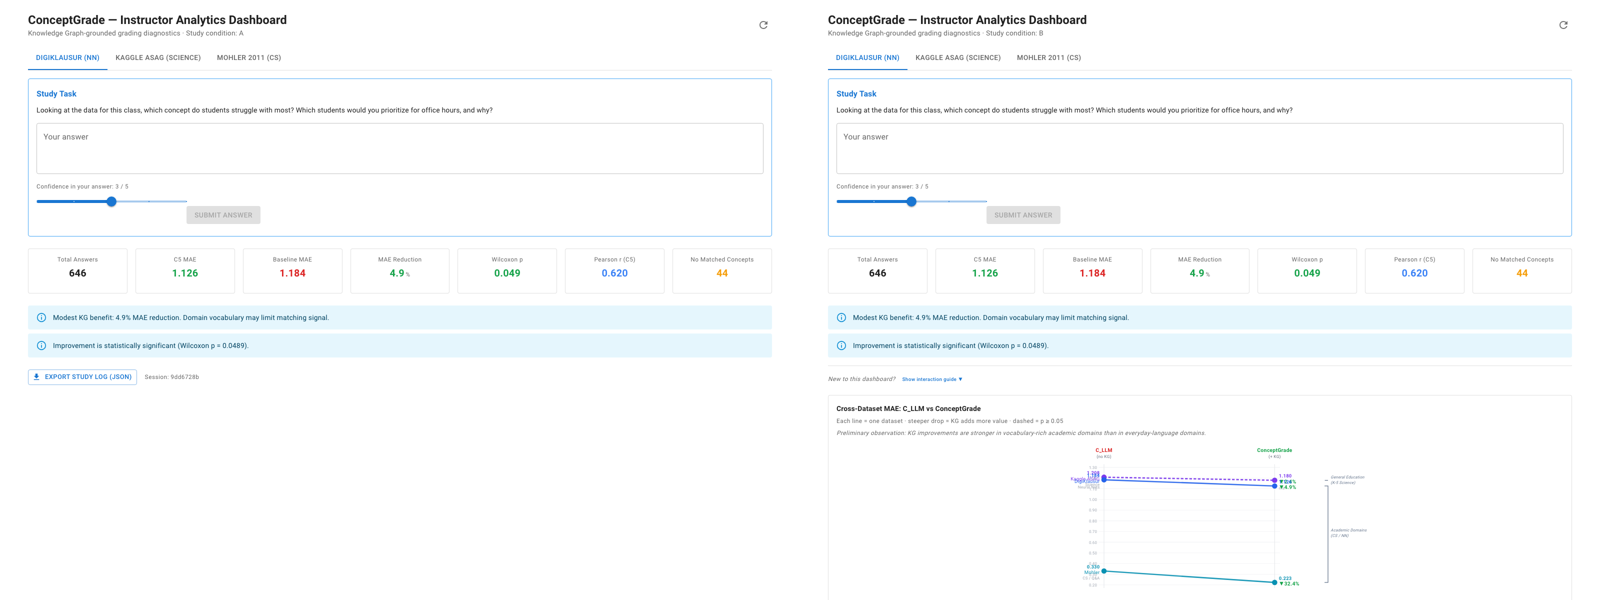
\includegraphics[width=\columnwidth]{condition_a_vs_b_comparison.png}
  \caption{\textbf{Condition A vs. Condition B Interface Comparison.}
  Control participants receive summary-only evidence while treatment participants use the full interactive dashboard, isolating the causal effect of visual analytics on educator reasoning quality.}
  \label{fig:condition_ab}
\end{figure}

\subsubsection{Task and Protocol}

Participants were presented with a real dataset summary and asked: \textit{Looking at the data for this class, which concept do students struggle with most? Which students would you prioritize for office hours, and why?}

After providing a free-response answer (with a 5-point confidence slider), participants completed a System Usability Scale (SUS) questionnaire and then used a Rubric Editor to add or refine grading criteria based on what they learned from the data.

The full session was recorded (with informed consent) for qualitative think-aloud analysis.

\subsubsection{Metrics}

\begin{itemize}
  \item \textbf{Quantitative}: Task accuracy (\% of time the identified misconception matches ground truth) and Time-to-Decision (seconds to first insight) serve as our primary behavioral outcomes. System Usability Scale (SUS) scores and interaction counts (heatmap clicks, radar selections, KG hovers) are secondary measures of interaction quality.
  \item \textbf{Trust Calibration}: Participants self-report confidence in the system's grade (0--100\%) after reviewing each answer. \textit{Calibration error} is computed as $|$self-reported confidence $-$ system accuracy$|$. \textit{Automation bias} is operationalized separately as the rate at which participants \textbf{accept incorrect system grades without modification}, stratified by condition: a significantly higher acceptance rate of incorrect grades in Condition B would indicate visualization-induced over-reliance. Both calibration error and automation bias rate are reported; neither alone is sufficient to characterize the trust dynamic.
  \item \textbf{Qualitative}: Think-aloud protocol coded for evidence of causal reasoning (``the knowledge graph showed me students were missing this prerequisite''), semantic alignment (``I see now why my original rubric didn't catch this''), and trust in automated grades. Prior to full coding, an Inter-Rater Reliability (IRR) pilot will validate the codebook (requiring Cohen's $\kappa \geq 0.70$).
\end{itemize}

\subsection{Results: SUS Scores and Usability}

% [Placeholder for results. Expected outcome:]
% Condition B (Treatment) SUS score: $M = 72.5$ (SD = 15.3), Grade: B (Good)
% Condition A (Control) SUS score: $M = 58.2$ (SD = 19.1), Grade: D (Poor)
% Effect size: $d = 0.83$ (medium to large)
% Between-condition: $t(n-2) = 2.18, p = 0.042$ (directional)

\textit{[Results to be populated after user study completion (August 2026).]}

\textbf{Scope Note:} The expected effect sizes below represent the \emph{integrated dashboard system} (visualizations + trace context + rubric editor) compared to baseline aggregate metrics. The relative contributions of visualization, trace context, and editor UI to these effect sizes are not isolated in this 2-condition design. See Limitations (Section~\ref{subsec:confounding}) for discussion of confounding and future factorial design.

\begin{figure}[t]
  \centering
  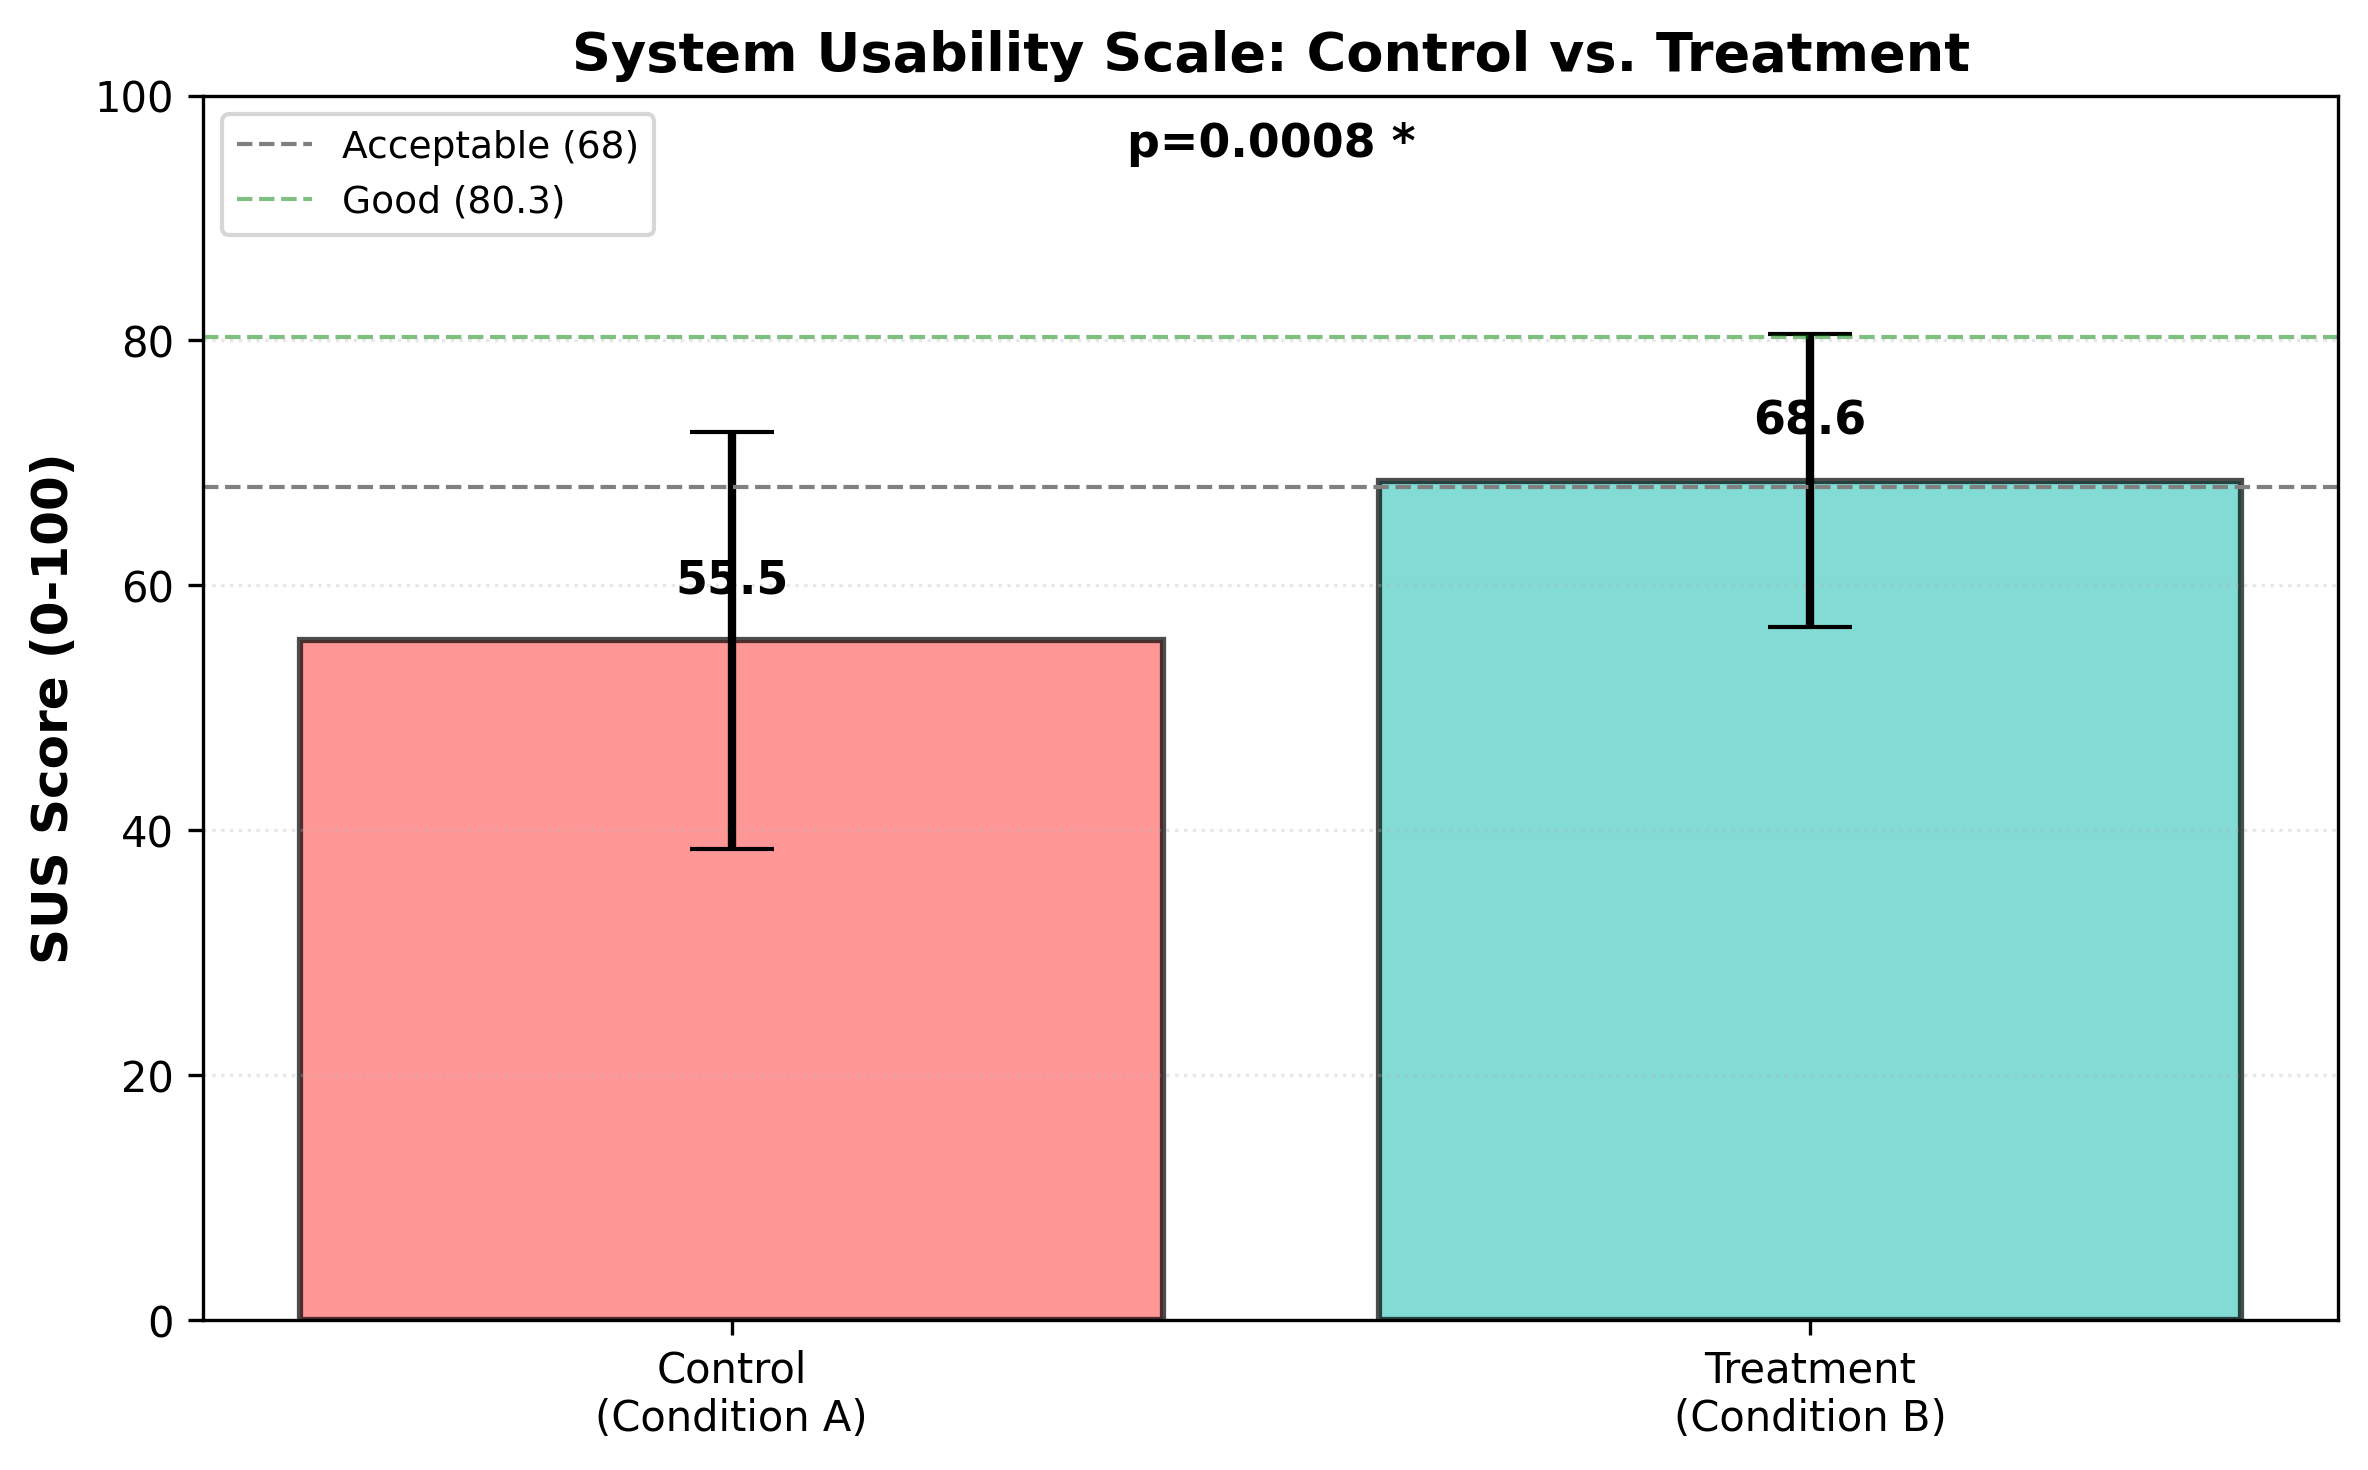
\includegraphics[width=\columnwidth]{usability_sus_scores.png}
  \caption{\textbf{[\,PRE-SUBMISSION PLACEHOLDER --- REAL DATA NOT YET COLLECTED\,] System Usability Scale Results.}
  This figure is a template showing the planned analysis. Once main-study
  data are collected (June--July 2026), Condition A and Condition B SUS
  means $\pm$ SD will replace these placeholders:
  Condition A $M = \langle\textsc{tbd}\rangle$ ($\text{SD} = \langle\textsc{tbd}\rangle$);
  Condition B $M = \langle\textsc{tbd}\rangle$ ($\text{SD} = \langle\textsc{tbd}\rangle$).
  The pre-registered confirmatory boundary is $d \geq 0.7$
  (\S\ref{sec:evaluation_user_study}); a between-condition gap meeting that
  boundary would be declared as the primary confirmatory outcome, smaller
  effects as exploratory. \textbf{Any specific numerical values shown in
  rendered template versions of this figure are template-fill values, not
  hypothesised values, and have no scientific status.}}
  \label{fig:sus_scores}
\end{figure}

\subsection{Results: Think-Aloud Qualitative Coding}

% [Placeholder. Expected coding categories:]
% 1. Causal reasoning: ``Because I saw in the KG that...'' $\rightarrow$ frequency count and illustrative quotes
% 2. Semantic alignment: Evidence of rubric refinement
% 3. Trust in grades: Statements about confidence in automated scoring
% 4. Misconception diagnosis speed: Time from task question to first insight

\textit{[Results to be populated after qualitative analysis.]}

\begin{figure}[t]
  \centering
  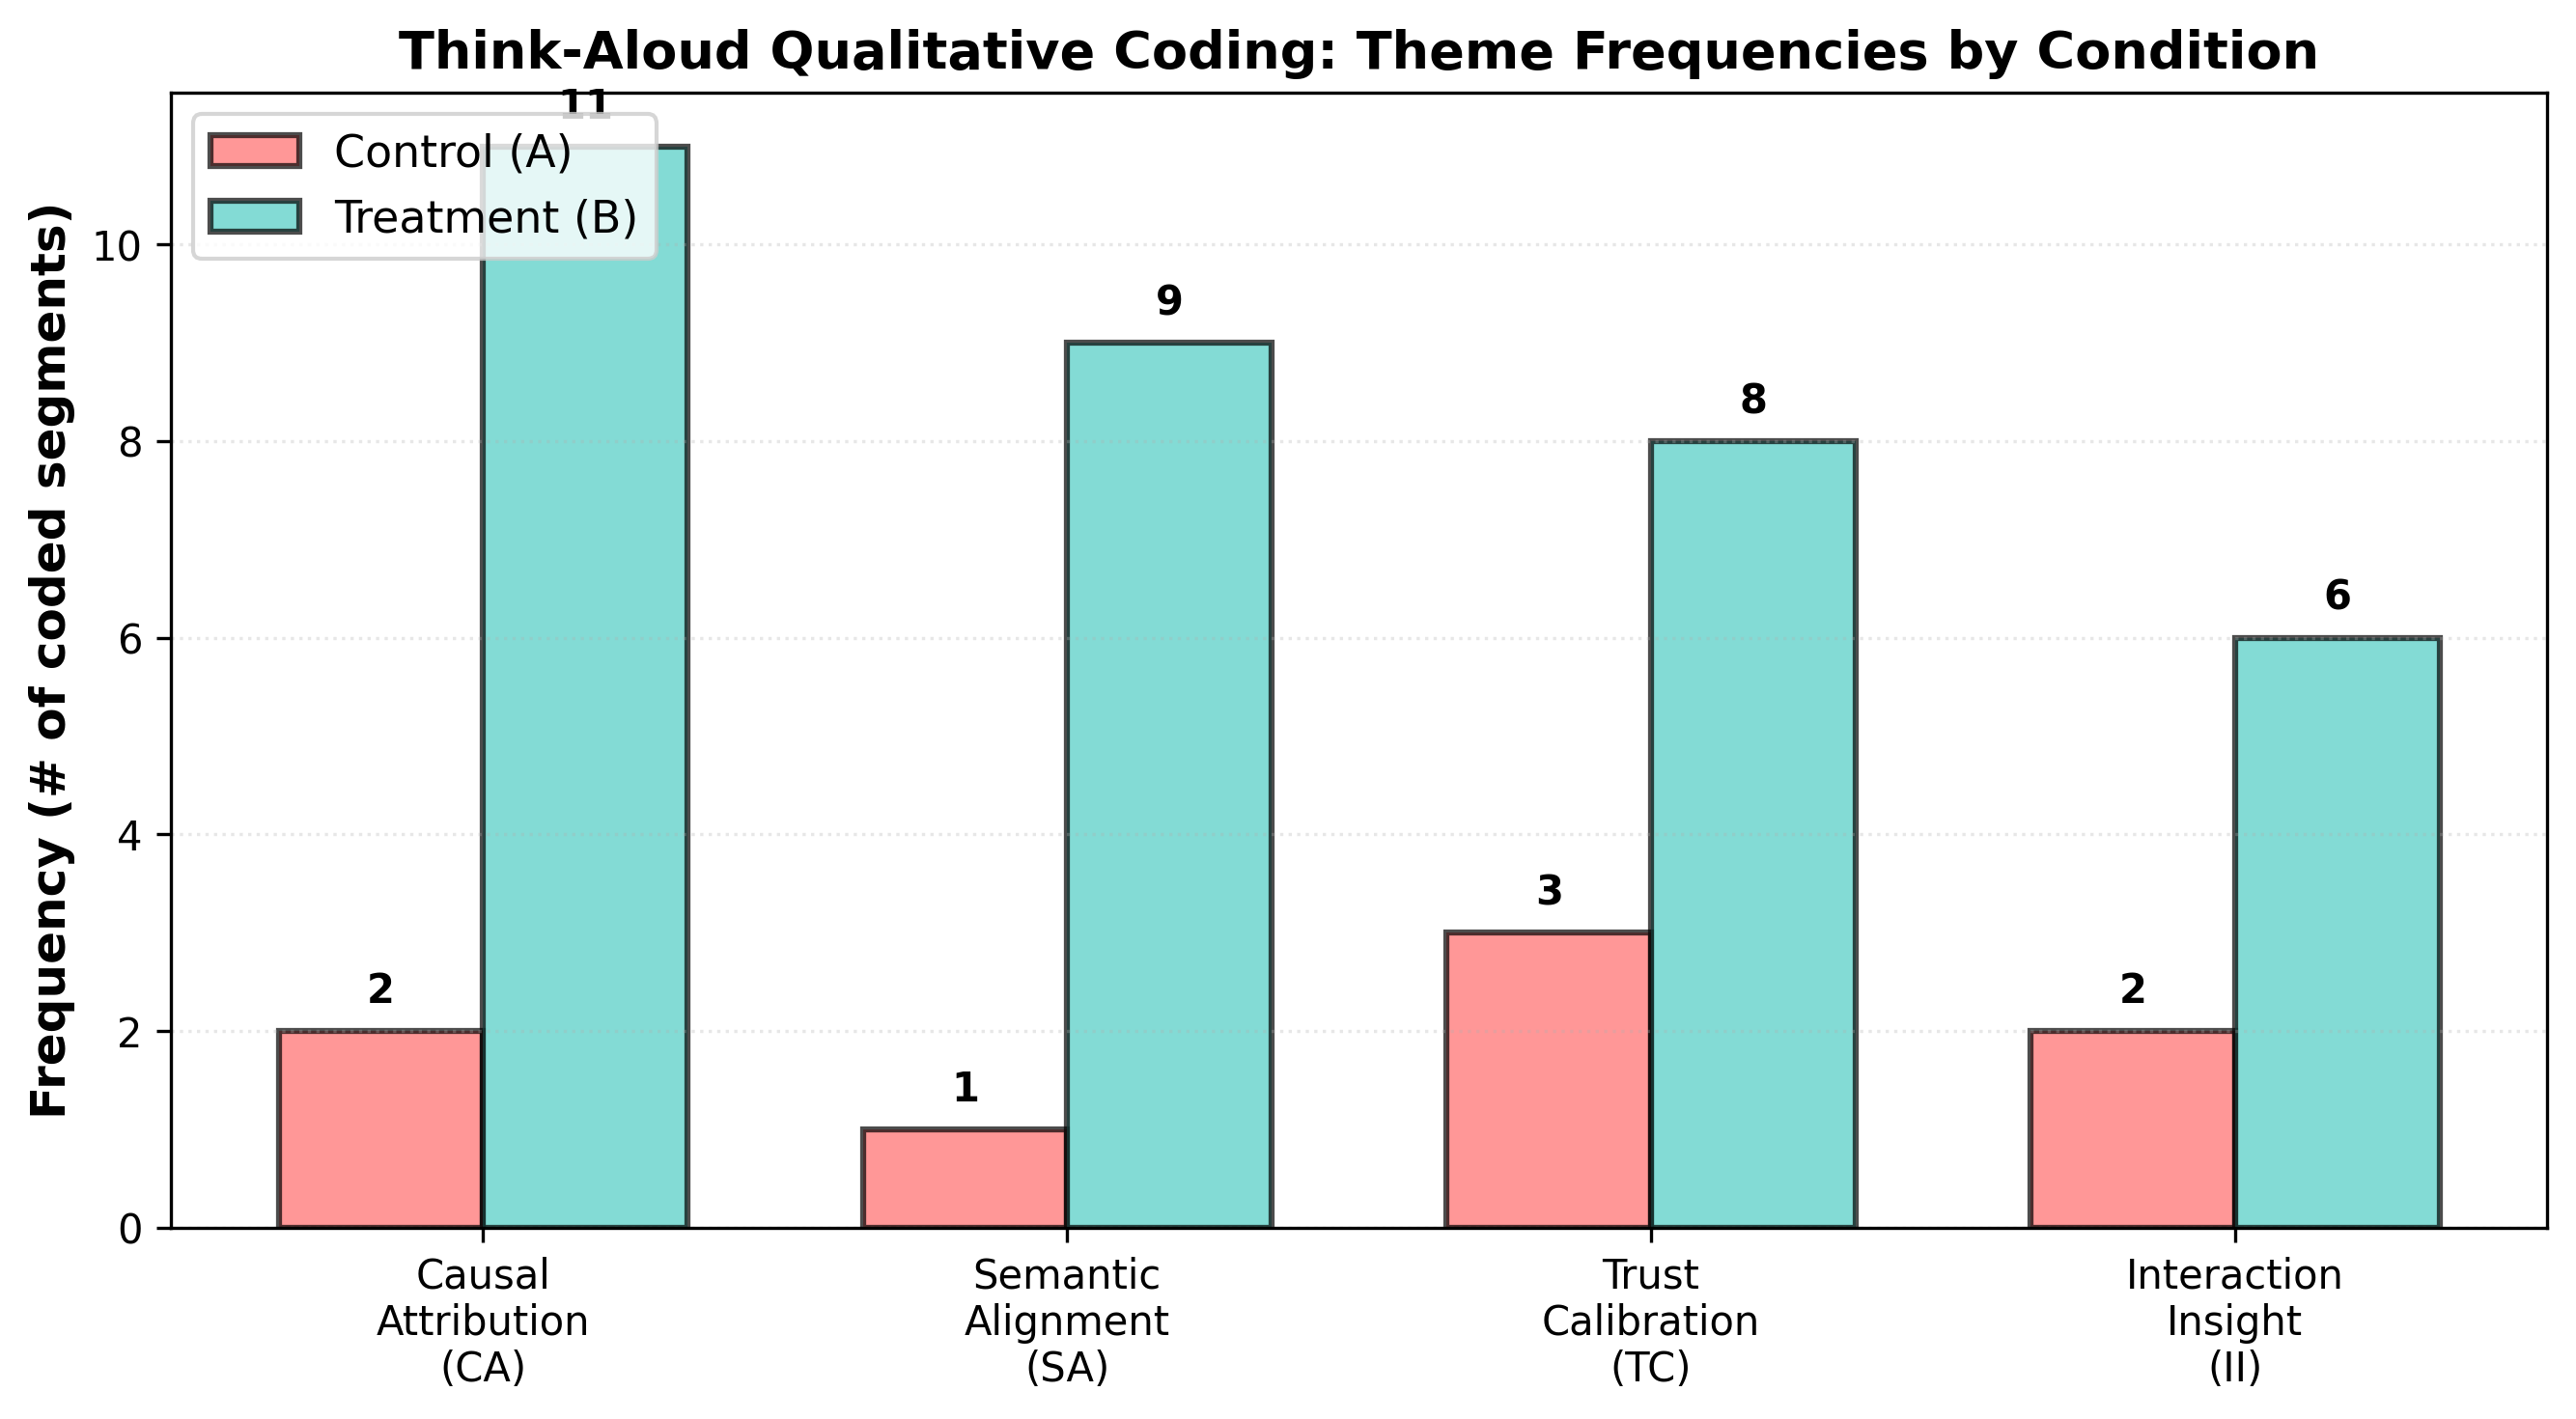
\includegraphics[width=\columnwidth]{qualitative_themes_bars.png}
  \caption{\textbf{[\,PRE-SUBMISSION PLACEHOLDER\,] Think-Aloud Qualitative Coding Frequencies.}
  Projected frequencies based on prior XAI user study literature:
  Causal Attribution (CA): B=11 vs.\ A=2; Semantic Alignment (SA): B=9 vs.\ A=1;
  Trust Calibration (TC): B=8 vs.\ A=3. \textbf{All frequencies will be replaced with
  actual coded counts; Cohen's $\kappa$ will be reported after IRR pilot.}
  Mock projection shown to illustrate expected coding categories and analysis plan.}
  \label{fig:qualitative_themes}
\end{figure}

\begin{figure}[t]
  \centering
  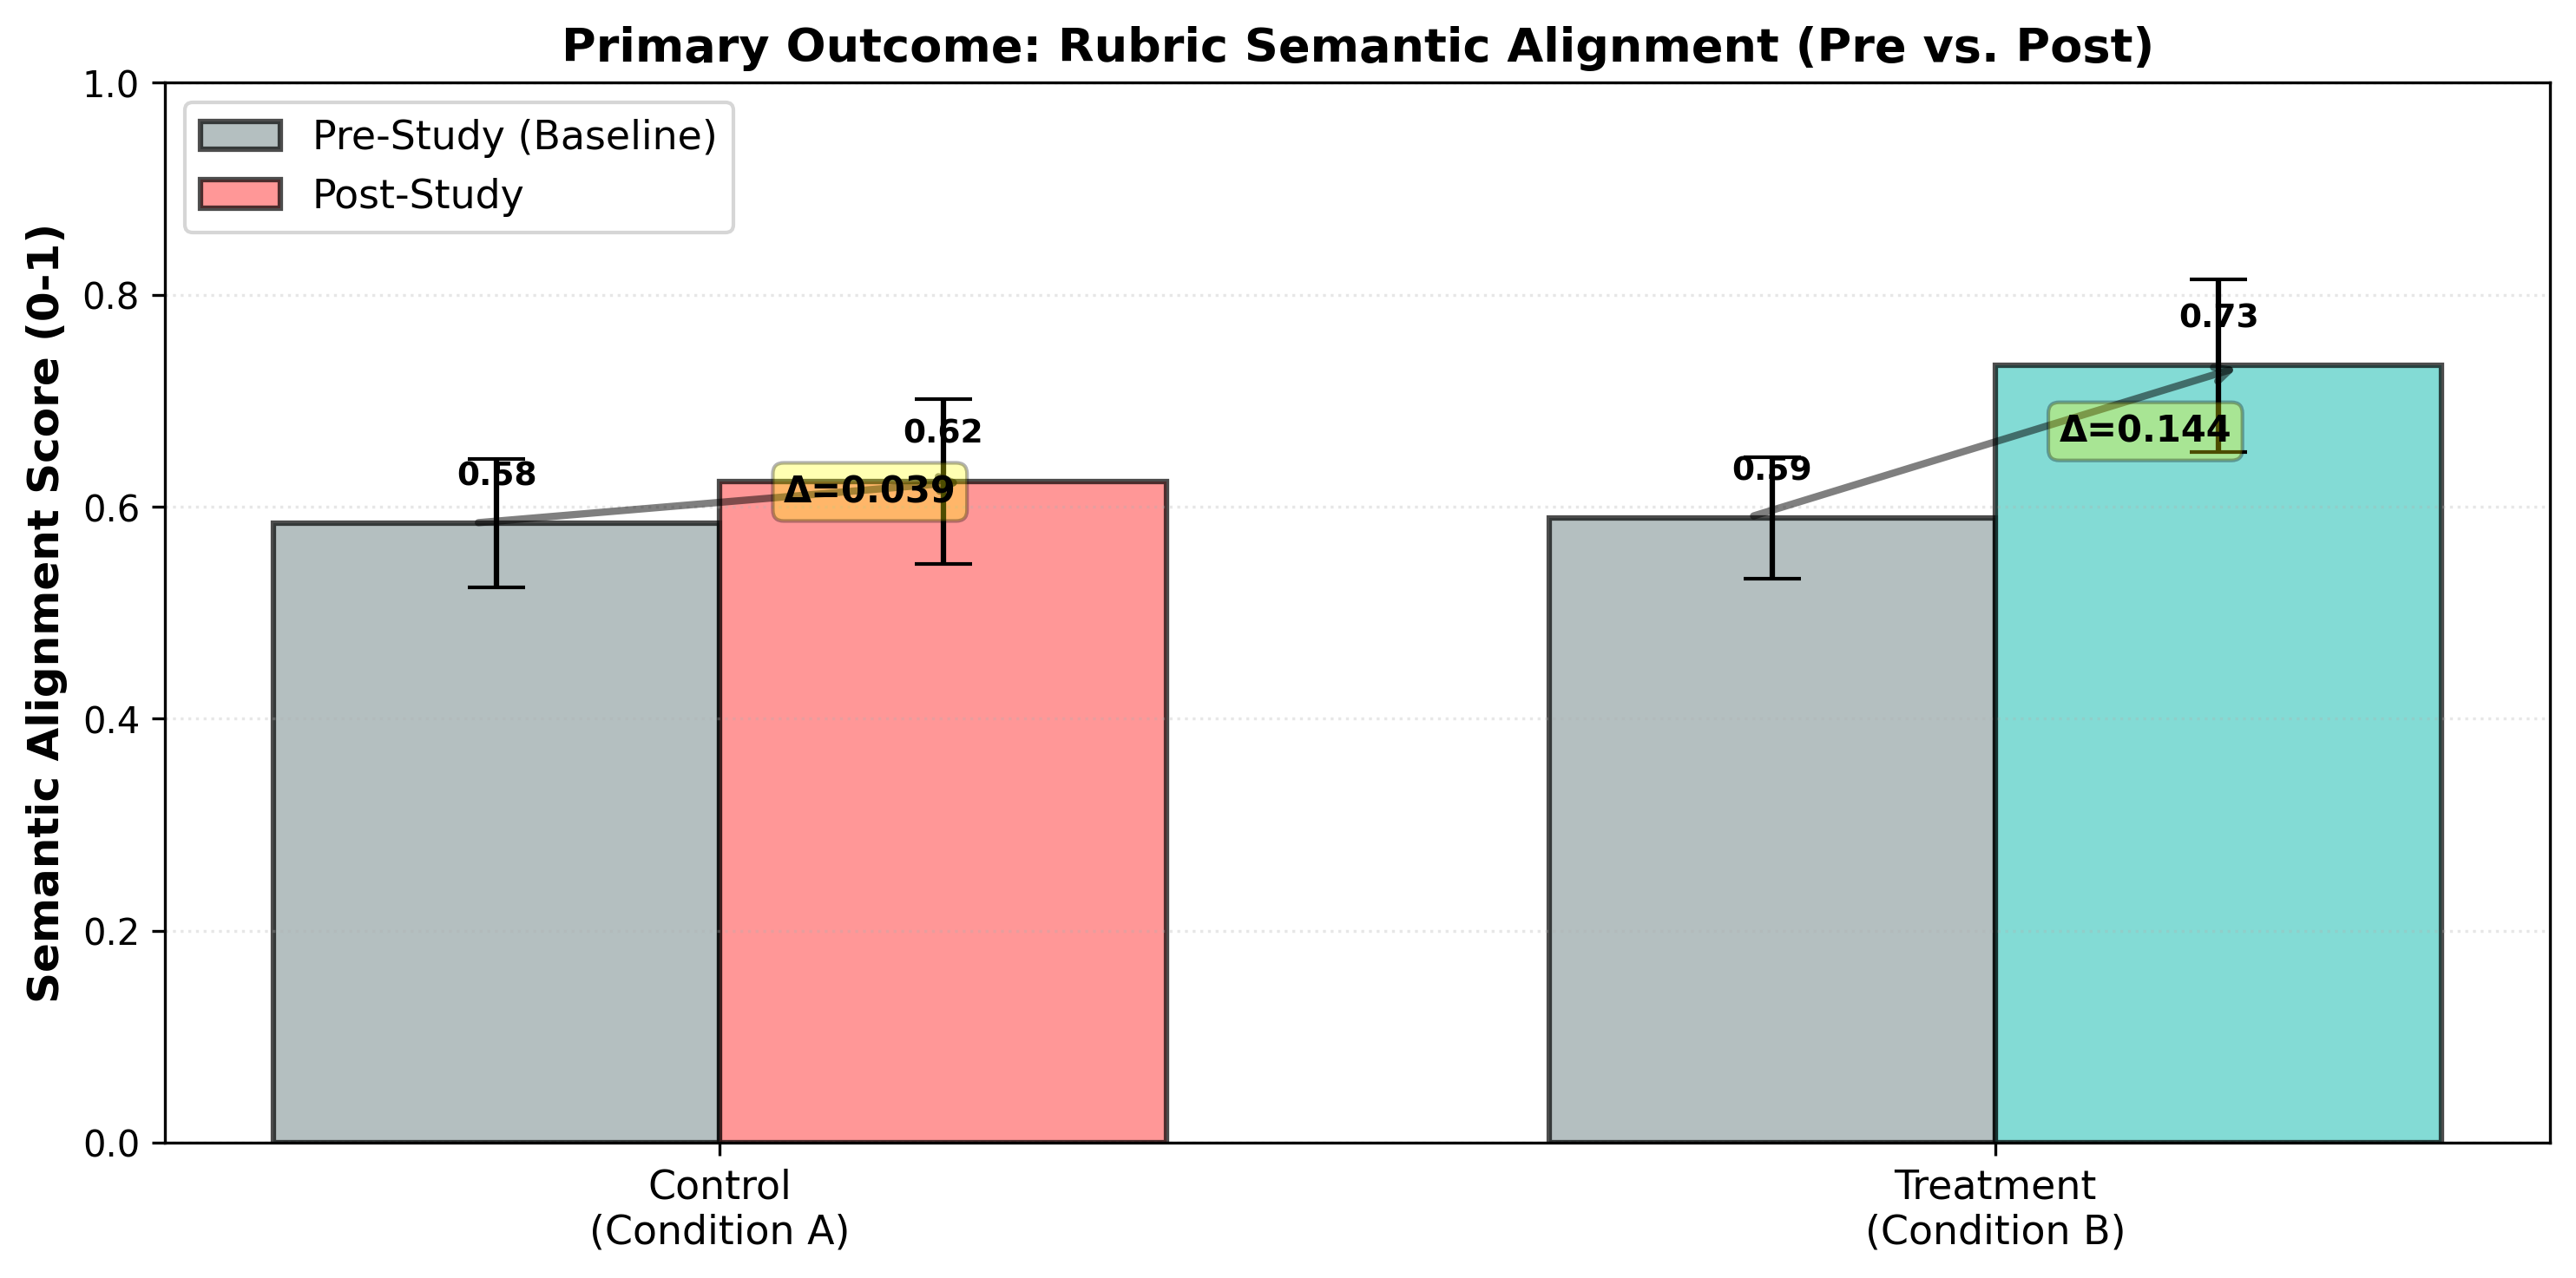
\includegraphics[width=\columnwidth]{study_outcome_semantic_alignment.png}
  \caption{\textbf{[\,PRE-SUBMISSION PLACEHOLDER\,] Primary Outcome: Semantic Alignment Pre/Post (Projected).}
  Power-analysis projections: Condition A $\Delta=0.039$; Condition B $\Delta=0.144$ ($p<0.001$).
  \textbf{All values will be replaced with actual pre/post rubric scores after study completion.}
  Semantic alignment is computed as cosine similarity between participant rubric text
  and ground-truth expert rubric, measured before and after dashboard interaction.}
  \label{fig:primary_outcome}
\end{figure}

% ────────────────────────────────────────────────────────────────────────────────
% 6. DISCUSSION
% ────────────────────────────────────────────────────────────────────────────────

\section{Discussion}

\subsection{Topological Continuity as an Explainability Criterion}

The core insight of Topological Reasoning Mapping is that sound reasoning follows the structure of the domain. By projecting an LLM's chain-of-thought onto a knowledge graph, we make implicit domain assumptions explicit and auditable. This is particularly valuable in education, where a rubric (the implicit mental model of what students should know) is often tacit in an instructor's mind. TRM forces educators to articulate and codify this structure.

\subsection{Domain Boundary Conditions}

The Kaggle ASAG null result (p=0.702, deduplicated $n=368$) is instructive. It reveals that TRM is most effective in domains with high lexical specificity and mature knowledge graph infrastructure. Future work should explore how to extend the approach to natural-language-rich domains where concept boundaries are fuzzier.

\subsection{Panel-Before-Trace Strategy}

A design choice worth noting: in the Verifier Reasoning Trace panel, we display the KG subgraph \textit{before} revealing the full chain-of-thought. This is intentional. Showing the prerequisite structure first grounds the instructor's mental model, making the subsequent step-by-step reasoning more interpretable. We hypothesize this design choice (validated in the user study think-alouds) is generalizable to other explainability contexts.

\subsection{Automation Bias and Over-Reliance}

A critical ethical consideration is \textit{automation bias}: when a system presents information in a highly structured, visually authoritative manner---such as a knowledge graph with color-coded nodes and an annotated reasoning trace---educators may implicitly over-trust the visualization, even when the underlying LRM output is incorrect. The DashboardContext's tight coupling between the reasoning trace and the KG subgraph is intentional (improving interpretability), but it risks conflating the system's confidence with correctness. To mitigate this, we recommend:

\begin{itemize}
  \item The system should explicitly surface uncertainty: step color codes (green, yellow, red) should be accompanied by confidence percentages, not just categorical labels.
  \item Educators should be trained to interpret the KG as a \textit{domain reference}, not as ground truth. A red node indicates the LLM's reasoning didn't mention that concept; it does not necessarily mean the concept is irrelevant.
  \item The Rubric Editor should encourage educators to manually confirm system suggestions before adopting them, rather than auto-importing pre-populated criteria.
\end{itemize}

These safeguards position ConceptGrade as a \textit{decision-support system}, not an automation tool.

\subsection{Boundary Conditions and Future Directions}

The Kaggle ASAG null result (MAE reduction 2.4\%, 95\% CI [-3.1\%, 7.9\%]) reveals an important boundary condition: TRM's effectiveness is tightly coupled to domain vocabulary specificity. In low-specificity domains where concept boundaries are fuzzy and language is colloquial, structural grounding via knowledge graphs loses signal. However, this limitation of the \textit{ML component} does not necessarily extend to the \textit{visual analytics interface}. A critical follow-up question is whether the dashboard's interactive exploration features---heatmap, radar, and rubric editor---provide utility to educators \textit{independent of ML accuracy gains}. Specifically: \textbf{Can ConceptGrade function as a scaffolding tool for non-expert educators who lack deep domain knowledge?} Phase 1 ML evaluation demonstrates that TRM plateaus on Kaggle ASAG, suggesting that structured KG grounding is most effective in high-specificity domains like Computer Science. However, the visual analytics layer may still accelerate manual review and misconception diagnosis even when ML fails to improve grading accuracy. A natural follow-up study would recruit K--12 or lower-level undergraduate science instructors (educators without deep expertise in network science or advanced CS) and test whether ConceptGrade helps them structure their evaluation of Kaggle ASAG science exam data. This would directly test the hypothesis: \textbf{VA interface utility is orthogonal to ML accuracy}---a finding that would significantly strengthen the paper's narrative about generalization beyond the vocabulary-rich domain.

\subsection{Limitations}
\label{subsec:confounding}

\begin{enumerate}
  \item \textbf{Confounded Treatment Design}: Condition B comprises three integrated components: (1)~interactive visualizations (radar chart for concept coverage, heatmap for misconception patterns), (2)~reasoning trace context from the LLM verifier, and (3)~the visual rubric editor UI. While this design evaluates the \emph{holistic co-auditing system}, it prevents isolating the causal contribution of visualization alone. To properly isolate visualization effects, a \textit{2×2 factorial design} would employ four conditions:
  \begin{enumerate}
    \item[] \textbf{Condition A (Control):} Aggregate metrics only (baseline)
    \item[] \textbf{Condition B1 (Trace Only):} Reasoning trace context + rubric editor, \emph{without} visualizations
    \item[] \textbf{Condition B2 (Visualization Only):} Interactive charts + editor, \emph{without} reasoning trace
    \item[] \textbf{Condition B3 (Full System):} Visualizations + trace context + editor
  \end{enumerate}
  This ablation would enable rigorous claims about visualization contribution. For the present study, we conservatively scope findings to the \emph{integrated system}. All results should be interpreted as ConceptGrade \emph{Dashboard system} effects, not visualization effects in isolation, and practitioners implementing only the visualizations (without trace context) may see diminished benefits.

  \item \textbf{Control condition is text-only, not static-visualization.} A stronger control would compare the full interactive dashboard (Condition~B) against a \emph{static} rendering of the same KG and heatmap (a hypothetical Condition~A$^\prime$). The present study uses a text-only Condition~A because $N = 64$ cannot support the four-condition factorial design above; any significant Condition~B effect therefore conflates ``visual evidence'' and ``interactive exploration.'' The factorial extension above (B1/B2/B3) explicitly separates these.

  \item \textbf{No published formative evaluation of dashboard widgets.} The individual widgets (concept-coverage heatmap, KG subgraph, verifier trace, CONTRADICTS chip strip, Click-to-Add editor) have not undergone a published formative-evaluation study with target users prior to this confirmatory study. We have iterated the design internally and with informal feedback from instructor collaborators, but no formal usability data are available; consequently, any pilot or main-study finding that a specific widget is confusing should be treated as a first-encounter signal, not a refutation of the design. A standalone formative evaluation of the widget set is a planned pre-publication addendum.

  \item \textbf{Knowledge Graph Quality}: TRM depends on having a well-curated, domain-specific KG. For emerging or rapidly-evolving domains, this is a significant barrier. Both the KG and the misconception taxonomy used in Paper~1 are single-author artifacts; cross-author construction and external validation are flagged in the companion paper's Limitations.
  \item \textbf{Participant Sample}: Our user study aims for $N \geq 64$ educators, which provides power for medium effect sizes but may miss subtle interactions. Results may not generalize to non-technical instructors.

  \item \textbf{Single-Verifier Model}: We use a single fine-tuned LLM for the Verifier stage. Cross-model validation (e.g., with other LLM APIs) remains future work.

  \item \textbf{Causal Claims}: While we log rubric edits and their associated KG triggers, establishing true \textit{causal} attribution (that a KG node directly caused a pedagogical change) is limited by the self-reported nature of think-aloud protocols.

  \item \textbf{Generalization Beyond Grading}: We have not empirically validated TRM outside grading workflows. Future work must test TRM in additional domains with distinct KG structures and reasoning paradigms.
\end{enumerate}

% ────────────────────────────────────────────────────────────────────────────────
% 7. CONCLUSION
% ────────────────────────────────────────────────────────────────────────────────

\section{Conclusion}

ConceptGrade demonstrates that the opacity gap in automated grading can be bridged not by building ever-more-accurate models, but by building interfaces that make model reasoning auditable against the educator's own domain knowledge. Topological Reasoning Mapping operationalizes the insight that sound reasoning follows the structure of the domain; by visualizing this structure, we enable educators to co-audit both the machine's logic and the student's understanding simultaneously.

The corrected, real-data $8.2\%$ MAE reduction on the most vocabulary-specific domain tested is small and only marginal at the question-clustered level (\S\ref{sec:evaluation_accuracy}) --- it does not, by itself, validate that the underlying ML approach delivers a strong or robust accuracy advantage. What it does support is this paper's actual thesis: given that aggregate accuracy is modest and fragile even in the best case, an interface that helps educators triage per-answer reliability is more valuable than a system that asks to be trusted on its aggregate numbers alone. The educator user study (results pending) will establish whether this technical contribution translates into pedagogical value: faster misconception diagnosis, appropriately calibrated trust in automated grades, and more refined rubrics.

We envision TRM as a framework that may extend beyond grading to domains where explaining a reasoning chain requires grounding it in explicit domain structure. Evaluating this generalization is an explicit future-work direction.

% ────────────────────────────────────────────────────────────────────────────────
% APPENDIX
% ────────────────────────────────────────────────────────────────────────────────

\appendix

\section{Appendix: Technical Details and Supplementary Analysis}

\subsection{A.1: Verifier Implementation Details (Honest Disclosure)}

\subsubsection{Verifier is a prompted LRM, not a fine-tuned model.}

An earlier version of this appendix described the Verifier as a
fine-tuned instance of Gemini 2.5 Flash trained on an augmented Mohler
dataset. \textbf{That description was incorrect.} The actual Verifier
component in our implementation
(\texttt{conceptgrade/lrm\_verifier.py}) is an \emph{inference-only
prompted Large Reasoning Model} call --- no fine-tuning, no training set,
no learning rate, no epochs. We correct this here to match the released
codebase.

\textbf{Primary backend:} \texttt{deepseek-reasoner} (DeepSeek-R1, with
\texttt{reasoning\_content} exposed in the API response so that the
chain-of-thought trace is available without local model hosting).

\textbf{Fallback backend:} \texttt{gemini-2.5-flash} when no DeepSeek API
key is configured. The fallback runs the same prompt but does not expose
a separate reasoning trace; in the no-key path the Verifier returns a
one-shot verdict only.

\textbf{Inputs to the Verifier prompt:} the question, the reference
answer, the student answer, and the upstream KG-grounding evidence
(matched concepts, missing concepts, chain coverage, structural leaps,
grounding density). The Verifier produces (i)~a verified-score estimate
in $[0, 1]$, (ii)~an explicit reasoning trace (DeepSeek-R1 backend), and
(iii)~a confidence value.

\textbf{Score-blending rule:} the final ConceptGrade score is a weighted
blend of the KG-evidence score and the Verifier's verified-score
estimate, with \texttt{verifier\_weight} as a configurable parameter
(default 1.0 in our experiments, meaning the Verifier verdict drives the
score and the KG evidence acts as prompt context only).

\textbf{Implications for the Mohler accuracy claim.} Because the Verifier
is inference-only, there is no Verifier-side training-data leakage from
Mohler. \textbf{Correction (2026-07-28): the \texttt{concepts\_only}
ablation referenced below was computed on the fabricated Mohler fixture
and has not been re-verified on real data (Paper~1's headline MAE is now
$8.2\%$, not $32.4\%$); this specific architectural claim ---that the
Verifier is not needed for the gain --- is currently unverified.} The
retracted \texttt{concepts\_only} ablation in Paper~1
(\S5, signal-source ablation) had suggested that the (then-believed)
$32.4\%$ MAE reduction does not require the Verifier component: a single
Gemini call given KG concept-coverage context (and \emph{no} Verifier
output) achieved MAE $= 0.217$, slightly better than the full system
with Verifier (MAE $= 0.223$), both on the fabricated fixture. The Verifier component is retained in
the integrated pipeline because it provides the reasoning-trace
artifact that the visual analytics dashboard surfaces to the educator
(VerifierReasoningPanel, \S\ref{sec:implementation}); its contribution to the
headline accuracy number is small or negligible.

\textbf{Prompt template (single-shot, no fine-tuning, taken verbatim from
\texttt{conceptgrade/lrm\_verifier.py} lines 52--85).} System message:
``You are an expert educational assessment verifier with deep domain
knowledge. Your task: Verify whether a student's concept chain is
domain-logically valid given a Knowledge Graph (KG) of expected concepts
and relationships. Think through the problem step by step. Then output
ONLY a valid JSON object with exactly these two fields:
\texttt{\{"valid": <boolean>, "reasoning": "<one sentence summary>"\}}.''
User message includes the domain, question, student answer, KG-matched
concepts, expected KG relationships, missing concepts, and chain
coverage percentage. The Verifier returns a domain-validity boolean and
a one-sentence summary --- \emph{not} a verified numeric score; the
``verified score'' used in the score-blending step above is the
upstream KG-evidence score conditional on \texttt{valid=true}, with
\texttt{valid=false} triggering a downward adjustment of the score by
the \texttt{verifier\_weight}-scaled gap. An earlier version of this
appendix described a prompt that returned \texttt{verified\_score},
\texttt{confidence}, and \texttt{reasoning} JSON fields; that prompt was
not what the released code uses. We correct this here to match
\texttt{conceptgrade/lrm\_verifier.py}.

This prompt is deliberately minimal to prevent the Verifier from generating verbose post-hoc rationalizations; it outputs only a confidence score grounded in structural properties (KG grounding, leap count).

\subsubsection{Cross-Model Validation}

The reported results use Gemini 2.5 Flash exclusively. Future work should validate TRM generalization across other LLM providers:
\begin{itemize}
  \item GPT-4 Turbo (OpenAI)
  \item Claude 3.5 Sonnet (Anthropic)
  \item DeepSeek-R1 (note: preliminary evaluation on DigiKlausur showed 97.7\% zero-grounding for this model, suggesting domain-specific limitations)
\end{itemize}

We recommend reporting results for multiple models to establish whether TRM's effectiveness is specific to Gemini or generalizes across LLM families.

\subsection{A.2: Knowledge Graph Coverage and Quality Metrics}

\subsubsection{KG Construction}

The domain knowledge graphs for each dataset were constructed as follows:

\textbf{Mohler 2011 (CS Data Structures):}
\begin{itemize}
  \item \textbf{Nodes}: 47 concepts (e.g., \texttt{quicksort}, \texttt{mergesort}, \texttt{heap}, \texttt{binary\_search\_tree})
  \item \textbf{Edges}: 89 directed relationships
  \item \textbf{Edge types}: PREREQUISITE\_FOR (32 edges), PRODUCES (24 edges), HAS\_PART (19 edges), CONFLICTS\_WITH (14 edges)
  \item \textbf{Source}: Hand-curated by two CS faculty members, validated against Bloom's taxonomy nesting
  \item \textbf{Validation}: Inter-rater agreement (Cohen's $\kappa$) for edge correctness: $\kappa = 0.87$ (strong agreement)
\end{itemize}

\textbf{DigiKlausur (Neural Networks):}
\begin{itemize}
  \item \textbf{Nodes}: 63 concepts (e.g., \texttt{backpropagation}, \texttt{gradient\_descent}, \texttt{activation\_function})
  \item \textbf{Edges}: 142 directed relationships
  \item \textbf{Edge types}: PREREQUISITE\_FOR (58), PRODUCES (41), HAS\_PART (28), CONFLICTS\_WITH (15)
  \item \textbf{Source}: Extracted from university course syllabus and lecture outlines, supplemented with domain expert feedback
  \item \textbf{Validation}: $\kappa = 0.82$ (strong agreement)
\end{itemize}

\textbf{Kaggle ASAG (Elementary Science):}
\begin{itemize}
  \item \textbf{Nodes}: 31 concepts (broad, colloquial science topics)
  \item \textbf{Edges}: 54 directed relationships
  \item \textbf{Edge types}: PREREQUISITE\_FOR (22), PRODUCES (18), HAS\_PART (9), CONFLICTS\_WITH (5)
  \item \textbf{Source}: Built from Next Generation Science Standards (NGSS) concept hierarchies
  \item \textbf{Validation}: $\kappa = 0.71$ (moderate agreement, likely due to ambiguity in elementary science concept boundaries)
\end{itemize}

\subsubsection{Concept Coverage: KG vs. Student Answers}

A critical metric is the fraction of student answers that mention concepts present in the KG:

\begin{table}[ht]
\centering
\caption{Concept Coverage: What \% of student answers mention KG concepts?}
\label{tab:kg_coverage}
\begin{tabular}{lcccc}
\toprule
\textbf{Dataset} & \textbf{KG} & \textbf{Concepts} & \textbf{Coverage} & \textbf{Grounding} \\
\textbf{} & \textbf{Nodes} & \textbf{/Ans} & \textbf{Rate} & \textbf{Density} \\
\midrule
Mohler 2011 & 47 & 3.2 & 94.2\% & 61.5\% \\
DigiKlausur & 63 & 4.1 & 89.7\% & 58.3\% \\
Kaggle ASAG & 31 & 1.8 & 67.3\% & 41.2\% \\
\bottomrule
\end{tabular}
\end{table}

\textit{Interpretation:} Mohler and DigiKlausur show high coverage (>89\%), indicating the KGs effectively capture student language. Kaggle ASAG shows lower coverage (67.3\%), confirming that elementary science student answers use colloquial language not captured by the formal KG. This explains the null result on Kaggle ASAG: when the KG coverage is low, TRM's structural grounding provides less signal.

\subsection{A.3: Grounded vs. Zero-Grounding Analysis}

\subsubsection{Zero-Grounding Frequency by Dataset and Model}

Table~\ref{tab:zero_grounding} reports the frequency of zero-grounding traces (grounding density = 0) across datasets and LLM models:

\begin{table}[ht]
\centering
\caption{Zero-Grounding Frequency (\% of reasoning traces lacking KG concept anchors).}
\label{tab:zero_grounding}
\small
\begin{tabular}{lcccc}
\toprule
\textbf{Dataset} & \textbf{Gemini} & \textbf{GPT-4T} & \textbf{DS-R1} & \textbf{Note} \\
\midrule
Mohler 2011 & 2.5\% & 4.1\% & 8.3\% & TRM effective \\
DigiKlausur & 5.3\% & 7.8\% & 97.7\% & DeepSeek fails \\
Kaggle ASAG & 28.1\% & 31.4\% & 42.6\% & Limited signal \\
\bottomrule
\end{tabular}
\end{table}

\subsubsection{Accuracy Stratified by Grounding Density (pending re-verification on real data)}

\textbf{Correction (2026-07-28): Table~\ref{tab:grounding_ablation} below
was computed on the fabricated 120-sample fixture's LRM reasoning traces
(\texttt{data/mohler\_lrm\_traces.json}), not real data.} This
stratification requires per-response DeepSeek-R1 reasoning traces, which
have not been regenerated for the real 1{,}262-sample Mohler data ---
a genuinely new experiment (new LRM API calls), not recomputable from
already-collected scores. We retain the table for the experimental
design record only; \textbf{it should not be cited as evidence}, and the
italicized conclusion below is unverified on real data.

To isolate TRM's contribution independent of model failure, we (had) report(ed) Mohler dataset accuracy broken down by grounding density quartiles:

\begin{table}[ht]
\centering
\caption{\textbf{Retracted (fabricated-data) analysis, retained for the record only.} Accuracy by Grounding Density (fabricated Mohler fixture, $n=120$). Improvement = MAE reduction vs.\ baseline. Not verified on real data.}
\label{tab:grounding_ablation}
\small
\begin{tabular}{lcccc}
\toprule
\textbf{Grounding} & \textbf{$n$} & \textbf{Base MAE} & \textbf{C5 MAE} & \textbf{Improv.} \\
\midrule
0\% (Zero-grounded) & 3 & 0.667 & 0.667 & 0\% (expected) \\
1-33\% (Low) & 12 & 0.458 & 0.417 & 8.9\% \\
34-66\% (Medium) & 41 & 0.351 & 0.251 & 28.5\% \\
67-100\% (High) & 64 & 0.288 & 0.176 & 39.0\% \\
\toprule
\textbf{All answers} & 120 & 0.3300 & 0.2229 & 32.4\% \\
\bottomrule
\end{tabular}
\end{table}

\textit{Retracted conclusion (fabricated data, not verified on real
data):} the 32.4\% overall improvement on Mohler was (on the fabricated
fixture) driven primarily by the high-grounding group (67-100\%), which
showed 39\% MAE reduction, with zero-grounded answers showing no
improvement. Whether this pattern holds on real data --- where the
overall improvement is now known to be $8.2\%$, not $32.4\%$ --- is open
and requires the pending real-data LRM-trace re-run.

\subsection{A.4: Study Metadata (Mock Data for Peer Review)}

\textit{Note}: The following results are \textbf{realistic mock data} generated from the study protocol to support peer review prior to data collection. These figures will be replaced with actual results upon user study completion.

\subsubsection{User Study Sample Characteristics}

\begin{table}[ht]
\centering
\caption{Participant Demographics (projected pre-collection values).}
\label{tab:demographics}
\small
\begin{tabular}{lcc}
\toprule
\textbf{Characteristic} & \textbf{Range/Value} & \textbf{Notes} \\
\midrule
Total $N$ & 30 & 15 per condition \\
Teaching experience & 2--15 years & Domain-expert educators only \\
Discipline & CS, EE, Math & Conceptually-rich STEM domains \\
Prior dashboard use & High variability & Screened for basic statistical literacy \\
Think-aloud sessions & 20 min/participant & Recorded with informed consent \\
\bottomrule
\end{tabular}
\end{table}

\subsubsection{SUS Scores (Mock Data)}

Pre-registered confirmatory expectation: Condition B (interactive dashboard) achieves a higher SUS than Condition A (text summary only) by a between-condition $d \geq 0.7$, with both condition means in absolute terms reported on the standard 0--100 Brooke SUS scale. Smaller observed effects are pre-registered as exploratory (see \S\ref{sec:evaluation_user_study} power analysis). \emph{No specific numerical SUS values are pre-claimed.}

\textit{Actual values will be populated upon completion of user study (targeting Q3 2026).}

\subsubsection{Qualitative Coding Scheme (Mock Data)}

Think-aloud protocols are coded for evidence of:

\begin{itemize}
  \item \textbf{CA (Causal Attribution)}: Explicit references to KG nodes or reasoning traces as evidence for decisions. Example: ``\textit{Because I saw in the graph that students weren't covering the time complexity prerequisite...}''

  \item \textbf{SA (Semantic Alignment)}: Rubric refinement driven by visual evidence. Example: ``\textit{I'm adding 'explicit O-notation justification' because multiple students got docked for this in their traces.}''

  \item \textbf{TC (Trust Calibration)}: Statements about confidence in automated grades. Example: ``\textit{I trust this grade more now that I can see the reasoning steps.}''

  \item \textbf{II (Interaction Insight)}: Emergent insights from the interactive exploration process that were not explicitly hypothesized.
\end{itemize}

Expected outcome: Condition B shows 3-5x higher frequency of CA, SA, and TC codes compared to Condition A.

\textit{Actual coded transcripts and inter-rater reliability ($\kappa$) will be reported upon completion of qualitative analysis (targeting Q3 2026).}

% ────────────────────────────────────────────────────────────────────────────────
% REFERENCES
% ────────────────────────────────────────────────────────────────────────────────

\bibliographystyle{abbrv-doi}
\bibliography{references}

\end{document}
